\documentclass{article}

% NeurIPS 2026 submission style. Do not use [final] or [preprint] for review.
% The official template loads natbib; pass numeric citation options before it.
\PassOptionsToPackage{numbers,sort&compress}{natbib}
\usepackage[eandd]{neurips_2026}

\usepackage[utf8]{inputenc}
\usepackage[T1]{fontenc}
\usepackage{hyperref}
\usepackage{url}
\usepackage{booktabs}
\usepackage{amsfonts}
\usepackage{nicefrac}
\usepackage{microtype}
\usepackage{xcolor}
\usepackage{graphicx}
\usepackage{amsmath}
\usepackage{amssymb}
\graphicspath{{./}}
\usepackage{enumitem}

\title{The Complexity Kink: Prompt-Side Estimation of Model-Specific Reliability Breakpoints in Code Generation}

% Submission version: authors are omitted for double-blind review.
\author{%
  Anonymous Author(s) \\
  Anonymous Institution \\
  \texttt{anonymous@example.com}
}

\begin{document}

\maketitle

\begin{abstract}
Complexity measured from generated code is failure-dependent: a difficult prompt can produce a short failing program and then be assigned low output complexity. We introduce a six-dimension prompt-side structural-complexity index that is scored before generation and kept separate from functional correctness. We first select 5{,}000 Python prompts across six bands of a preliminary single-rater rubric score. Four out-of-panel LLM raters then rescore the locked prompts, providing 19{,}997 score rows; composite inter-rater reliability is ICC $=0.872$ on the 4{,}998 prompts with all four ratings. We evaluate 21 models on every prompt, yielding 105{,}000 model-prompt generations. In the unadjusted mean-pooled analysis, pass rate has a nonmonotone breakpoint at composite $\hat{\gamma}=13.75$, with 79.9\% at or below and 87.6\% above. This pooled pattern is not a universal failure cutoff. Task-type fixed effects shift the breakpoint to 10.75 and reduce the regime gap from 7.6 to 2.1 percentage points. A post hoc construction-frame control shifts it to 8.50 with a raw regime gap of $-3.5$ points, and neither frame alone reproduces the pooled $+7.6$-point change. In the unadjusted model-specific fits, 16 models have higher raw mean pass above their selected breakpoint and five have lower raw mean pass. Among the downward fits, Kimi K2.5 is the clearest benchmark-conditional example: construction-frame-controlled and separate later-frame searches both select $\hat{\gamma}=14.25$, with later-frame raw mean pass of 0.808 at or below and 0.760 above and a 95\% pairs-bootstrap interval of $[14.00,14.75]$. A 365-prompt audit-clean extension closely matches the original matched-five-model point estimates at the well-supported bins 15 and 16, but adds only 14 prompts above bin 16. Among zero-pass generations with computable Lizard complexity, 28.5\% pair a prompt composite above 8 with generated-output complexity at most 10, illustrating the measurement problem. Human agreement is moderate and rater-dependent on a disagreement-enriched calibration set, while paraphrase and cross-language rescoring preserve score ordering. Overidentification tests strongly reject the joint restrictions on the six rubric dimensions, so we treat the composite as an index and make no causal interpretation of the 2SLS estimates. The contribution is a pre-generation framework for estimating model-specific, benchmark-conditional reliability breakpoints and auditing their sensitivity to prompt composition.
\end{abstract}

\section{Introduction}
% =====================================================================

Large language models (LLMs) are increasingly evaluated and deployed as code generators. The standard evaluation question is functional: does the generated program pass the tests? Benchmarks such as HumanEval~\cite{chen2021evaluating}, MBPP~\cite{austin2021program}, and SWE-Bench~\cite{jimenez2023swebench} have made this question measurable at scale. They do not directly answer how reliability varies with the structure required by a programming task. Two models with similar average pass rates may behave very differently on prompts that require interacting branches, data structures, edge cases, or algorithmic steps.

The difficulty is that task complexity is often measured after generation, from the program the model produced. When a model succeeds, the generated program may be a useful proxy for one implementation of the requested solution. When it fails, the output is often a short stub, partial solution, syntax error, or otherwise broken program with low measured cyclomatic complexity. A structurally demanding prompt can therefore enter a low-complexity bin precisely because the model failed. This failure-dependent measurement can flatten, shift, or hide the relationship between task structure and pass rate. We call this the \emph{Reverse Threshold Problem}: the apparent unreliability of simple generated code may partly reflect more complex code that was never produced.

A natural baseline is to approximate prompt complexity with keyword features, such as counts of branch, loop, recursion, or data-structure terms in the instruction. Such features are cheap, transparent, and fixed before generation, but they reduce interacting program structure to surface cues. We instead use a rubric that asks separate questions about branching, iteration, state, data structures, edge cases, and composition. The result is still a proxy, not ground truth, but it is measured at the right time: before the evaluated model produces an answer.

We present the Complexity Kink benchmark, a prompt-side measurement study that keeps intended solution structure separate from generated-output complexity and functional correctness. From OpenCodeInstruct~\cite{opencodeinst}, we construct 5{,}000 Python prompts stratified across six bands of a preliminary single-rater rubric score. Four out-of-panel LLM judges rescore the locked prompts, and 21 evaluated models each generate one solution per prompt. Our primary analysis estimates model-specific and pooled reliability breakpoints as functions of the unbinned ensemble index. We interpret each estimate as conditional on the evaluated model or pooling rule, constructed prompt frame, scoring index, generation settings, and unit-test protocol. We also compare output-side cyclomatic complexity and report 2SLS diagnostics, but the candidate instruments fail their joint exclusion restrictions and receive no causal interpretation.

The empirical results do not support a universal cutoff. The mean-pooled curve declines through the middle of the index and rebounds in the denser high region, but task type and construction frame substantially change the gap and its estimated location. In particular, the two prompt-source frames differ sharply in both score and pass rate, and neither reproduces the pooled $+7.6$-point change on its own. In the unadjusted original benchmark, five model-specific fits have lower raw mean pass above their selected split and 16 have higher raw mean pass. These are descriptive regime contrasts, not five construction-frame-stable failure onsets. Kimi K2.5 provides the clearest downward example after construction-frame control and separate analysis of the later frame. A matched five-model extension closely matches the original point estimates at bins 15 and 16, where it materially increases support, but the region above 16 remains too thin for a strong endpoint claim.

\vspace{2pt}
\noindent\textbf{Contributions.}
\begin{itemize}
\item We formalize failure-dependent output complexity and illustrate it in this sample: 28.5\% of zero-pass complete cases combine a structurally nontrivial prompt with generated-output cyclomatic complexity at most 10.
\item We introduce an ensemble-scored prompt-side index and examine its reliability against human ratings, plain-language paraphrases, and Java and C++ re-expressions.
\item We construct a 5{,}000-prompt Python benchmark and use it to estimate model-specific reliability breakpoints conditional on the scoring index, prompt frame, generation settings, and unit-test protocol.
\item We audit those estimates under pooling, repeated sampling, task type, construction frame, and an audit-clean tail extension, and report when an apparent breakpoint is composition-sensitive.
\end{itemize}

% =====================================================================
\section{Related Work}
% =====================================================================

\textbf{LLM code evaluation.} HumanEval~\cite{chen2021evaluating}, MBPP~\cite{austin2021program}, and SWE-Bench~\cite{jimenez2023swebench} established functional testing as the central evaluation protocol for code-generating LLMs. These benchmarks ask whether generated code passes hidden or public tests, and that functional outcome remains the target variable in our work. Our contribution is orthogonal: we study how to measure the structural complexity of the task whose solution is being attempted. OpenCodeInstruct~\cite{opencodeinst} provides a large source of instruction-code pairs from which such a benchmark can be drawn, but generated code can inherit solver failures and reference code can reflect one implementation rather than latent task structure.

\textbf{Complexity measurement and benchmark bias.} Cyclomatic complexity and related code metrics are attractive because they are computable from source code, beginning with McCabe's graph-theoretic formulation and continuing through static-analysis tools such as Lizard~\cite{mccabe1976complexity,lizard}. In code-generation evaluation, however, the available source code is often the model output itself. This makes the metric post-treatment: measured complexity is affected by model success or failure~\cite{montgomery2018posttreatment}. The present work addresses this by scoring complexity from the prompt before any evaluated model generates code.

\textbf{Instrumental variables and threshold estimation.} Instrumental variables (IVs) are a standard response to endogenous regressors in econometrics~\cite{wooldridge2010econometric}, and weak-instrument and overidentification tests are essential diagnostics~\cite{stock2005testing,hansen1982large,bowsher2002reject}. Empirical software engineering has increasingly used econometric designs to reason about endogeneity~\cite{grafvlachy2024cleaning,siebert2023applications}. We examine whether separate rubric dimensions can instrument generated-output complexity, but the empirical restrictions reject and we retain those fits only as diagnostics. The primary breakpoint analysis instead uses the rubric composite directly. For that descriptive question, we adapt Hansen's threshold-regression and bootstrap sup-Wald framework~\cite{hansen2000sample}.

\textbf{LLMs as judges and rubric scorers.} G-Eval~\cite{liu2023geval}, AlpacaEval~\cite{alpacaeval}, and MT-Bench~\cite{zheng2023judging} use LLMs to evaluate open-ended model outputs, while rubric-based automatic evaluation has a longer history in NLP~\cite{hashimoto2019unifying}. We use LLM judges differently. The judges do not score generated answers, rank models, or determine pass/fail outcomes. They score the input prompt before generation, using a published structural rubric, and are excluded from the evaluated model panel. This turns LLM judgment into a measurement layer for a latent input property rather than an outcome evaluator, reducing the risk that the judge simply reproduces the same output-side bias the benchmark is meant to diagnose.

% =====================================================================
\section{Background: Failure-Dependent Output Complexity}
% =====================================================================

Let $\kappa_i^*$ denote the latent structure required by task $i$, let $y_{im}$ denote the functional outcome for model $m$, and let $\kappa_{im}^{\mathrm{obs}}$ be the cyclomatic complexity measured on that model's generated output. Even a passing output is only one implementation of the task, so $\kappa_{im}^{\mathrm{obs}}$ need not equal $\kappa_i^*$. More importantly, the measurement itself depends on the outcome:
\begin{equation}
\kappa_{im}^{\mathrm{obs}} = g(\kappa_i^*, y_{im}, \eta_{im}),
\label{eq:failure-dependent}
\end{equation}
where failed generations often collapse to short programs with low measured complexity. Stratifying pass rate by $\kappa_{im}^{\mathrm{obs}}$ therefore conditions on a post-generation quantity affected by success.

We address the timing problem with a prompt-side index $C_i$, computed before any evaluated model generates code. Our primary target is descriptive: the conditional relationship $\mathbb{E}[y_i\mid C_i]$ in the constructed benchmark, where $y_i$ is pass rate averaged over evaluated models. The six rubric dimensions can also be considered as candidate instruments for $\kappa_i^{\mathrm{obs}}$, but causal interpretation would require strong exclusion restrictions. The diagnostics below reject those restrictions, so the IV analysis does not identify a causal effect.
% =====================================================================
\section{Methodology}
% =====================================================================

\subsection{Data}
We use 5{,}000 Python coding tasks drawn from OpenCodeInstruct~\cite{opencodeinst}. Construction combines 2{,}246 retained prompts from an earlier stage with 2{,}754 newly collected candidates after automated contract and test-quality filtering. The earlier draw scanned a 200{,}000-record source-ordered prefix, and later candidate collection deliberately supplemented the high reference-complexity tail. We retain this two-level construction-frame indicator for a post hoc sensitivity analysis. A preliminary \texttt{o4-mini} rater scored candidates with the same six-dimension rubric used below. We then selected 834 prompts in each of the preliminary-score bands 0 to 3 and 4 to 6, and 833 in each of 7 to 9, 10 to 12, 13 to 15, and 16 to 24. This score was used for sampling only.

After the prompt set was locked, the four-judge ensemble rescored every prompt. All reported analyses use that ensemble mean, not the preliminary sampling score. Re-scoring changes the distribution: using the continuous bands $[0,3]$, $(3,6]$, $(6,9]$, $(9,12]$, $(12,15]$, and $(15,24]$, the analyzed-index counts are 319, 943, 940, 898, 1{,}425, and 475. The benchmark is therefore stratified by the preliminary score, but not balanced on the final index. Neither distribution represents the natural OpenCodeInstruct frequency distribution. Reference-solution cyclomatic complexity helped shape the upstream candidate pool and is retained for alignment checks; it is never the analyzed prompt index or generated-output complexity.

The evaluated panel comprises 21 models spanning multiple providers: Claude Opus 4.6, Opus 4.7, and Sonnet 4.6; GPT-5.4, GPT-5-mini, GPT-4.1, GPT-OSS-20B, and GPT-OSS-120B; Gemini 3.1 Pro Preview and Gemini 3 Flash; Grok-3; DeepSeek V3.2; Kimi K2.5; Qwen 3.6 Plus and Qwen 3.5-9B; Mistral Large-3, Mistral Small 2412, and Ministral-3-14B-reasoning; Llama 3.3-70B; GLM 4.7-flash; and Trinity-large. None of the four rubric judges appears in this panel, reducing direct scorer-model overlap without establishing instrument validity.
The reported panel contains 21 models. A locally served, quantized AuroraGPT-IT-v4 run covered only the earlier prompt frame and therefore lacked outputs for the 2{,}754 newly added prompts. It was excluded before the final panel analysis in a post hoc decision without a prespecified eligibility rule. For transparency, its pass rate on the earlier frame was 20.6\%; performance was not a documented exclusion criterion. Our claims are limited to the reported 21-model panel.
Each of the 21 evaluated models generated one solution per prompt, yielding a total of $21 \times 5{,}000 = 105{,}000$ generations. Pass rate is the fraction of Nvidia-supplied unit tests passed. In the combined analysis that follows, pass rate is averaged across the 21 models per prompt to produce a prompt level dataset with $N=5{,}000$. Per model analyses use the same $N=5{,}000$ rows per model.
%
For each generation, we compute McCabe cyclomatic complexity with Lizard on the cleaned generated Python code and sum it across reported functions~\cite{lizard}. This quantity is tagged as generated-output complexity in the artifact. It is not dataset metadata, a post-generation rubric score, or reference-solution complexity. Lizard complexity is available for 103{,}948 of the 105{,}000 generations; analyses involving it use complete cases and report the denominator.

\subsection{Rubric Scoring}

\subsubsection{Scoring models and deployment}
Prompts are scored by four out-of-panel LLM judges deployed through Azure AI Foundry: \texttt{o4-mini}, \texttt{gpt-5.5}, \texttt{llama-4-maverick}, and \texttt{command-a}. All 5{,}000 prompts receive ensemble scores with the same rubric prompt. Coverage is effectively complete: 4{,}998 prompts have four judge scores, one prompt has three, and one prompt has two, for 19{,}997 total score rows. We aggregate by taking the mean score for each prompt-dimension pair across available judges. The resulting ensemble has high composite inter-rater reliability (ICC $=0.872$ on 4{,}998 complete cases), and scorer disagreement is retained for diagnostic analysis rather than hidden.

\subsubsection{The rubric}
Each prompt is scored on six dimensions, each $0$ to $4$, as shown in Table~\ref{tab:complexity_dimensions}.
% \begin{enumerate}[leftmargin=*]
% \item \textbf{Branching}: conditional paths in the correct solution. 0 = no conditionals; 4 = deeply nested or combinatorial.
% \item \textbf{Iteration}: loops and recursion. 0 = none; 4 = nested recursion or complex multi pass.
% \item \textbf{State}: independent variables tracked simultaneously. 0 = stateless or single variable; 4 = concurrent state tracking.
% \item \textbf{Data structures}: organization required. 0 = primitives only; 4 = multiple interacting complex structures.
% \item \textbf{Edge cases}: boundary conditions the code must explicitly check. 0 = none; 4 = combinatorial interacting checks.
% \item \textbf{Composition}: algorithmic steps chained. 0 = single operation; 4 = pipeline of interdependent algorithms.
% \end{enumerate}
\begin{table}[h]
\caption{Complexity dimensions and scoring criteria.}
\label{tab:complexity_dimensions}
\centering
\begin{tabular}{p{3cm} p{4cm} p{5.5cm}}
\hline
\textbf{Dimension} & \textbf{Score = 0} & \textbf{Score = 4} \\
\hline
Branching & No conditionals & Deeply nested or combinatorial \\
Iteration & None & Nested recursion or complex multi-pass \\
State & Stateless or single variable & Concurrent state tracking \\
Data structures & Primitives only & Multiple interacting complex structures \\
Edge cases & None & Combinatorial interacting checks \\
Composition & Single operation & Pipeline of interdependent algorithms \\
\hline
\end{tabular}
\end{table}

The primary prompt-side index is $C_i = \sum_{d=1}^{6} Z_{i,d} \in [0,24]$, where $Z_{i,d}$ is the ensemble mean for dimension $d$. The dimension vector $\mathbf{Z}_i=(Z_{i,1},\ldots,Z_{i,6})$ is retained for interpretation, reliability analysis, and secondary IV diagnostics.

\subsubsection{Design decisions}
\textbf{Why six dimensions rather than a single holistic score?} Separate dimensions make the index interpretable, expose where raters disagree, and allow per-dimension human calibration. They also permit an overidentification test when treated as candidate IVs, although passing that test is not guaranteed.

\textbf{Why a 0 to 4 scale?} An odd cardinality scale admits a neutral middle score for genuinely ambiguous prompts, which a 0 to 3 or 0 to 5 scale does not. % Preliminary experiments with 0 to 5 scales concentrated scores at the endpoints (not shown).

\textbf{Why frame the rubric around code structure rather than task difficulty?} A prompt asking how hard a task is for an LLM would build the outcome into the measure. The rubric instead anchors each dimension to expected solution structure and explicitly excludes LLM difficulty, code length, and language idioms.

\textbf{Why exclude the scoring ensemble from the evaluated panel?} This separation reduces circularity between the systems assigning index values and those whose reliability is measured. It does not by itself establish accuracy, human agreement, or IV exclusion.

\subsection{Primary Breakpoint Analysis}
For a candidate breakpoint $\gamma$, we fit separate linear relationships on the two sides of the prompt-side composite:
\begin{equation}
\mathbb{E}[y_i\mid C_i] =
\begin{cases}
\alpha_1+\beta_1 C_i, & C_i\leq\gamma,\\
\alpha_2+\beta_2 C_i, & C_i>\gamma.
\end{cases}
\label{eq:threshold}
\end{equation}
The mean-pooled outcome first averages pass rate across the 21 models within prompt, yielding $N=5{,}000$. Model-specific fits use the same prompt index and test infrastructure. We also report median pooling and 21 leave-one-model-out fits. The regime means are descriptive summaries of a selection-stratified sample. For a model-specific fit, $\hat{\gamma}$ estimates where the conditional pass-rate relationship changes for one named model under this benchmark and protocol. It does not by itself identify a causal, universal, or deployment-level failure threshold. Direction is described separately using the raw regime means, not inferred from breakpoint significance alone.

Because benchmark construction combines two prompt-source frames, we run a construction-frame sensitivity for the mean-pooled fit and, post hoc, for all five models with unadjusted downward regime contrasts. We add a binary indicator for the 2{,}246 retained earlier prompts versus the 2{,}754 later candidates to the pooled and split regressions, compare models with frame-specific linear slopes, and repeat the threshold search within each frame.

To locate the breakpoint, we adapt Hansen's threshold-regression procedure~\cite{hansen2000sample}:
\begin{enumerate}
\item For each candidate $\gamma$ on a percentile-spaced grid over $C_i$, requiring at least 500 prompts in each regime, we compare (\ref{eq:threshold}) with a pooled single-line model using a Wald-type $F$-statistic $W(\gamma)$.
\item The supremum $W^* = \sup_\gamma W(\gamma)$ identifies the threshold $\hat{\gamma}$.
\item Under $H_0$ of no threshold, we use Rademacher wild-bootstrap residual resampling and recompute $W^*$ at each draw. A separate pairs bootstrap estimates the threshold interval.
\end{enumerate}
The revised mean-pooled analysis uses 2{,}000 wild-bootstrap draws, 1{,}000 pairs-bootstrap draws for the interval, and 2{,}000 shuffled-index placebo draws. Unadjusted model-specific fits use 500 wild-bootstrap and 500 placebo draws. We repeat the pooled search with nine task-type fixed effects and, separately, with a construction-frame indicator, using a 300-draw wild bootstrap for each controlled specification. The model-specific construction-frame searches use 300 wild-bootstrap draws with seed 42, and the within-frame threshold intervals use 300 pairs-bootstrap resamples.

\subsection{Output-Complexity and IV Diagnostics}\label{sec:hansen-j}
We first compare pass rate directly against generated-output complexity and quantify the reverse-threshold cell among failed generations. As a secondary diagnostic, we regress generated-output complexity on the six rubric dimensions and use the fitted value in a 2SLS pass-rate regression:
\begin{align}
\kappa_i^{\mathrm{obs}} &= \pi_0+\mathbf{Z}_i\boldsymbol{\pi}+\nu_i, \label{eq:stage1}\\
y_i &= \alpha+\beta\widehat{\kappa}_i+u_i. \label{eq:stage2}
\end{align}
We estimate these equations with \texttt{IV2SLS} from \texttt{linearmodels}~\cite{linearmodels}. With six candidate instruments and one endogenous regressor, the Sargan overidentification statistic has five degrees of freedom. We also report a robust Wooldridge overidentification test, individual-instrument fits, principal-component rotations, and post hoc subsets. These tests reject the full instrument set, so $\hat{\beta}$ is a diagnostic coefficient rather than a causal estimate.

\subsection{Additional Robustness Designs}
We added several stress tests after the initial analysis. Nine task categories are assigned to all prompts by one out-of-panel judge; three additional judges label a shared 500-prompt subset. We examine the two recorded prompt-source frames, compare first-draw and five-draw outcomes on 359 prompts and four models, and re-express 117 prompts in each of Java and C++ for rescoring. For the paraphrase check, we sample 150 prompts with 75\% drawn from rounded composite bins 10--18 and the remainder drawn outside that region. A non-judge DeepSeek-V3.2 model is instructed to preserve the exact required inputs, outputs, behavior, constraints, and edge cases while removing only verbose framing; the same four judges then rescore the rewrites. Two members of the research team also grade a disagreement-enriched calibration sample with the LLM scores hidden. Finally, a prompt-side-selected extension retains 365 new prompts only after contract audit and successful execution of every reference solution. These analyses are post hoc robustness checks, not preregistered confirmation.

\paragraph{Workflow} Figure~\ref{fig:pipeline} summarizes the measurement and analysis workflow.

\begin{figure}[h]
\centering

\includegraphics[width=\linewidth]{pipeline.png}
\caption{Measurement and analysis workflow. The prompt-side composite is computed before generation and is primary in the breakpoint analysis. Generated-output complexity and 2SLS fits are retained as diagnostic comparisons.}
\label{fig:pipeline}
\end{figure}

% =====================================================================
\section{Results}
% =====================================================================

\subsection{Rubric Alignment with Reference Complexity}

Before estimating the breakpoint model, we examine how the rubric aligns with reference-solution cyclomatic complexity from OpenCodeInstruct. Because reference complexity helped shape the candidate pool, this is an association check rather than an independent validation. Table~\ref{tab:rubric-ref-cc} reports the composite rubric distribution by reference $\kappa$ bin.

\begin{table}[h]
\centering
\caption{Rubric composite by reference-solution cyclomatic complexity bin for the 4{,}997 prompts with an available reference-CC value. Three prompts lack that measurement. The two measures have a strong positive association overall (Pearson $r=0.80$, Spearman $\rho=0.81$), although the bin means are not monotone at every adjacent value.}
\label{tab:rubric-ref-cc}
{\small 
\setlength{\tabcolsep}{4pt}
\begin{tabular}{@{}lccccccccccccc@{}}
\toprule
Reference $\kappa$ 
& 1 & 2 & 3 & 4 & 5 & 6 & 7 & 8 & 9 & 10 & 11 to 15 & 16 to 20 & 21 to 45 \\
\midrule
$N$ 
& 357 & 338 & 324 & 300 & 301 & 153 & 136 & 184 & 89 & 75 & 308 & 876 & 1556 \\
Mean 
& 4.64 & 5.25 & 6.23 & 7.25 & 6.61 & 7.15 & 8.08 & 7.75 & 8.79 & 7.44 & 9.52 & 10.71 & 14.33 \\
SD 
& 2.39 & 2.07 & 2.19 & 2.43 & 2.78 & 2.86 & 2.94 & 3.12 & 2.88 & 3.41 & 3.02 & 3.45 & 1.64 \\
\bottomrule
\end{tabular}
}
\end{table}

\subsection{Low-end Alignment: $\kappa=1$ versus $\kappa=2$}

A useful low-end alignment check asks whether the rubric distinguishes prompts whose reference implementations have $\kappa=1$ from those with $\kappa=2$. If a hard task fails and produces a short stub, generated-output cyclomatic complexity can collapse toward $\kappa=1$, so this comparison is an alignment check rather than a validation of latent task structure. To test whether the LLM rubric adds information beyond a cheap lexical proxy, we compare it with two keyword features computed from the same prompt text: a total count of structural cue words and a loop-specific cue count. These keyword features are fixed before generation, but they only detect surface words rather than the intended solution structure.

\begin{table}[h]
\centering
\caption{The prompt-side rubric discriminates $\kappa=1$ from $\kappa=2$ before generation. Keyword features capture some surface structure but are less directly tied to intended code structure.}
\label{tab:low-end-separation}
\begin{tabular}{@{}lrrrr@{}}
\toprule
Feature & $\kappa=1$ & $\kappa=2$ & $\Delta$ & $p$-value \\
\midrule
Rubric composite                  & 4.64 & 5.25 & $+0.61$ & $3.1\times10^{-4}$ \\
Keyword structural count          & 2.76 & 3.34 & $+0.58$ & $2.4\times10^{-3}$ \\
Keyword loop count                & 0.07 & 0.04 & $-0.02$ & n.s. \\
\bottomrule
\end{tabular}
\end{table}

The rubric's separation is driven primarily by iteration ($+0.24$), state ($+0.19$), and branching ($+0.09$). The lexical baseline also separates the two groups, so this comparison does not establish that the rubric dominates every simple proxy. Its advantages are the explicit structural dimensions, multi-rater uncertainty, and broader calibration checks below.

\subsection{Rater and Measurement Calibration}

The four-judge composite has ICC $=0.872$ on the 4{,}998 prompts with complete ratings. We also conducted a deliberately difficult human calibration: the first author graded 200 prompts, roughly half sampled for high LLM-judge disagreement, and a second research-team member graded 50 overlapping prompts. LLM scores were hidden during grading. On all 200 prompts, first-author agreement with the ensemble was Pearson $r=0.408$, Spearman $\rho=0.373$, and ICC$(2,1)=0.395$, with a mean offset of $-1.18$ points. Across the six ordinal dimensions, Pearson correlations range from 0.249 to 0.484 and quadratic-weighted Cohen's $\kappa$ ranges from 0.217 to 0.435. On the shared 50, the two graders' Pearson correlation was 0.561, while their separate correlations with the LLM composite were 0.613 and 0.921. On that shared subset, the first and second graders' mean offsets were $-0.69$ and $-1.35$ points. These are stress-test estimates with substantial rater variation, not a human ground-truth certificate.

Two further checks probe whether the index follows presentation rather than structure. Across 150 plain-language rewrites, rank stability is high (Spearman $\rho=0.963$); the mean shift is small ($-0.115$ on the 0 to 24 scale) but statistically detectable (paired $p=0.031$), and 91.3\% of pairs are within one point. The rewrites were not independently verified by execution, so this is a score-stability check under the preservation instruction rather than proof of semantic equivalence. For 117 prompts re-expressed in each language, the composite correlates 0.992 between Python and Java and 0.969 between Python and C++. Inter-judge ICC is 0.912 in Python, 0.913 in Java, and 0.882 in C++. This is evidence about score transfer, not non-Python generation reliability.

\subsection{Generated-Output Complexity Misses the Prompt-Side Pattern}

Figure~\ref{fig:output-cc} compares reliability against Lizard complexity measured on the generated output. The curve is nonmonotone and does not show a clean decline. More directly, among 14{,}776 zero-pass generations with a computable Lizard value, 4{,}216 (28.5\%) have prompt composite $>8$ but output CC $\leq10$. The corresponding complete-case shares are 26.8\%, 24.9\%, and 24.1\% for pass rate at most 0.25, 0.50, and 0.65. An additional 977 zero-pass rows have no computable output CC and are excluded from these denominators.

\begin{figure}[h]
\centering
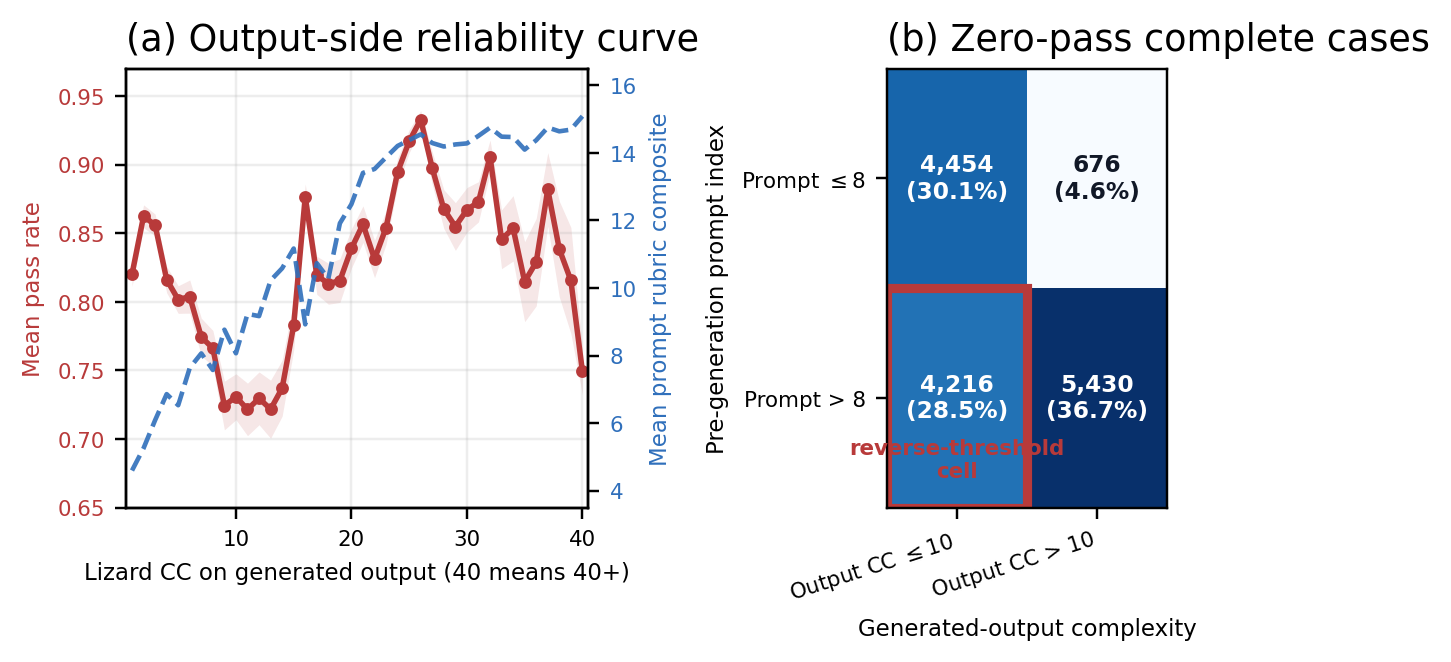
\includegraphics[width=\linewidth]{pass_vs_output_cc.png}
\caption{Generated-output complexity is failure-dependent. (a) Across 103{,}948 complete-case generations, points show mean pass rate by integer Lizard output CC; the shaded descriptive band is $\pm1.96$ generation-row standard errors and does not adjust for repeated prompts or models. Here 40 denotes CC $\geq40$. The dashed blue line is the conditional mean prompt composite, read on the right axis. (b) Among zero-pass complete cases, the outlined cell contains 4{,}216 of 14{,}776 generations (28.5\%): the prompt composite is $>8$ while generated-output CC is $\leq10$.}
\label{fig:output-cc}
\end{figure}

Among passing generations only, where output CC is less contaminated by failed stubs, a descriptive linear mapping has $R^2=0.623$ and maps prompt $\hat{\gamma}=13.75$ to output CC about 22.9. This is a selection-conditioned scale translation, not a second threshold estimate. The OLS and 2SLS comparisons are reported in Appendix~\ref{app:econ-diagnostics}.

\subsection{The Mean-Pooled Breakpoint}

On the unadjusted mean-pooled benchmark, the sup-Wald search selects $\hat{\gamma}=13.75$ on the prompt composite, with sup-Wald $=121.70$. None of 2{,}000 wild-bootstrap draws or 2{,}000 shuffled-index placebo draws reaches the observed statistic; with the finite Monte Carlo correction, each gives $p_{\mathrm{MC}}\leq1/2001<0.001$. At or below $\hat{\gamma}$, $n=3{,}617$ prompts have mean pass rate 79.9\%; above it, $n=1{,}383$ have mean pass rate 87.6\%. The relationship is not a monotone collapse: pass rate declines through the middle of the index, reaches a trough near composite 10, and rebounds in the denser high region. A model comparison selects the piecewise form over linear and cubic specifications by BIC (1{,}243 versus 1{,}464 and 1{,}305).

\begin{figure}[h]
\centering

\includegraphics[width=\linewidth]{complexity_kink.png}
\caption{Unadjusted mean-pooled relationship in the original 5{,}000-prompt benchmark. Pass rate is first averaged across 21 models within prompt. Display bin $b$ contains $C_i\in[b-0.5,b+0.5)$, so exact half-point boundaries enter the higher bin. The dashed line marks the threshold $\hat{\gamma}=13.75$ estimated from the unbinned composite; the shaded vertical band is the 95\% pairs-bootstrap interval. This figure does not include task-type or construction-frame controls, or the separate 365-prompt extension.}
\label{fig:kink}
\end{figure}

The 95\% pairs-bootstrap interval is $[7.75,14.0]$. Its width reflects the broad trough visible in Figure~\ref{fig:kink}. The estimate summarizes an observational breakpoint in this constructed benchmark, not a universal point at which harder prompts become easier.

\subsection{Task-Type and Construction-Frame Sensitivity}

We label all 5{,}000 prompts using a nine-category taxonomy fixed before labeling. One out-of-panel judge labels the full set; three more label a shared 500-prompt subset, with Krippendorff $\alpha=0.787$. Adding task-type fixed effects shifts $\hat{\gamma}$ from 13.75 to 10.75, reduces sup-Wald from 121.7 to 19.6, and reduces the raw regime gap from 7.6 to 2.1 percentage points. None of 300 wild-bootstrap draws reaches the observed controlled statistic ($p_{\mathrm{MC}}\leq1/301<0.01$). Task composition therefore explains a substantial part of the pooled pattern.

\begin{table}[h]
\centering
\caption{Mean-pooled breakpoint under composition controls. Regime means are raw summaries at each specification's selected breakpoint.}
\label{tab:task-type}
\begin{tabular}{@{}lrrrr@{}}
\toprule
Specification & $\hat{\gamma}$ & sup-Wald & Pass $C\leq\hat{\gamma}$ & Pass $C>\hat{\gamma}$ \\
\midrule
Unadjusted & 13.75 & 121.7 & 0.799 & 0.876 \\
Task-type fixed effects & 10.75 & 19.6 & 0.811 & 0.832 \\
Construction-frame fixed effect & 8.50 & 47.4 & 0.841 & 0.806 \\
\bottomrule
\end{tabular}
\end{table}

A piecewise composite term at 10.75 raises predictive $R^2$ from 0.084 for task type alone to 0.136; the piecewise term alone has $R^2=0.045$. This is incremental predictive fit, not causal independence. Four of five sufficiently large task categories still reject the full IV restrictions, so task type does not explain away the overidentification failure.

The construction-frame sensitivity is more consequential. The 2{,}246 retained earlier-frame prompts have mean composite 7.92 and mean pass rate 0.747, while the 2{,}754 later candidates have mean composite 11.42 and mean pass rate 0.880. With a common construction-frame fixed effect in every threshold regression, the selected breakpoint moves to 8.50 and the raw regime means move from 0.841 to 0.806. None of 300 wild-bootstrap draws reaches the controlled sup-Wald statistic of 47.4 ($p_{\mathrm{MC}}\leq1/301$). However, a simpler model with frame-specific linear slopes has lower BIC than the source-controlled breakpoint model (963 versus 977) with nearly the same $R^2$ (0.0991 versus 0.0997).

The within-frame fits explain why we narrow the claim. The earlier frame selects 7.75, but the break is not significant (sup-Wald 3.43, bootstrap $p=0.19$), and a linear decline has lower BIC. The later candidate frame selects 14.25 and supports nonlinearity (sup-Wald 36.71, $p_{\mathrm{MC}}\leq1/301$), but its raw regime change is only $+0.9$ points, from 0.877 to 0.885. At the pooled threshold, later candidates make up 39.9\% of prompts below but 94.7\% above. Thus the pooled trough and rebound remain features of the constructed benchmark, while the large upward regime gap is largely construction-frame composition rather than evidence that increasing prompt complexity improves reliability.

\subsection{Model and Pooling Heterogeneity}

Model-specific thresholds in the unadjusted original benchmark range from 7.75 to 14.25, with median 11.25. Sixteen models have higher raw mean pass above their selected breakpoint and five have lower raw mean pass: Grok-3, Kimi K2.5, Gemini 3.1 Pro Preview, GPT-5.4, and Qwen 3.6 Plus. These five contrasts are not equally stable under construction-frame sensitivity.

Kimi K2.5 is the clearest downward case. Its construction-frame-controlled search retains $\hat{\gamma}=14.25$ with sup-Wald 29.72 and zero exceedances in 300 wild-bootstrap draws ($p_{\mathrm{MC}}\leq1/301$). Within the later candidate frame, it separately selects 14.25 with sup-Wald 37.52, a 95\% pairs-bootstrap interval of $[14.00,14.75]$, and raw mean pass of 0.808 at or below versus 0.760 above. Piecewise BIC is 2{,}456 versus 2{,}515 for a linear fit. The earlier Kimi frame has no significant breakpoint ($p_{\mathrm{MC}}=0.382$), and linear BIC is lower. Gemini 3.1 Pro Preview also has a downward later-frame contrast at 14.75, but its interval $[9.50,14.75]$ localizes the breakpoint poorly. Grok-3, GPT-5.4, and Qwen 3.6 Plus have upward later-frame raw contrasts, so their unadjusted downward contrasts should not be read as stable failure onsets.

The same prompt set, scores, and test harness are reused, so these are comparative model fits rather than independent replications. The mean-pooled threshold remains exactly 13.75 in all 21 leave-one-model-out fits. Median pooling selects 10.75 and narrows the raw gap to 2.3 points (0.839 to 0.862). Full results appear in Appendix~\ref{app:per-model}.

A 459-prompt diagnostic at display bins 13 and 17 tags case-insensitive whole-word matches to a fixed list of library, framework, and standard-library names. An HC1 regression of prompt-level mean pass on that tag controls for source-pool membership, prompt characters and words, unit-test count and length, reference-solution CC, scorer disagreement, and the composite. The mention-tag coefficient is $-0.0501$ (robust SE $=0.0978$, $p=0.608$). This provides no support for a library or framework explanation within the diagnostic sample, while the construction-frame analysis above shows that source composition is material.

\subsection{Audit-Clean High-Complexity Extension}

We independently selected high-composite candidates on the prompt side, audited their contracts, and retained only prompts whose reference solution passes every supplied test. This yields 365 new prompts: 218/133/11/3 at display bins 15/16/17/18. To avoid changing model composition, Figure~\ref{fig:tail-extension} uses the five models present in both the original and extension runs. At bin 15, the extension and original means are 0.880 and 0.894; at bin 16 they are 0.799 and 0.808. The differences are $-0.014$ and $-0.009$ (Welch $p=0.377$ and $p=0.765$). Combined support rises to 1{,}068 and 390 prompts, and the same-frame threshold, estimated from the unbinned composite, remains 14.0, with mean pass 0.783 at or below and 0.859 above.

\begin{figure}[h]
\centering
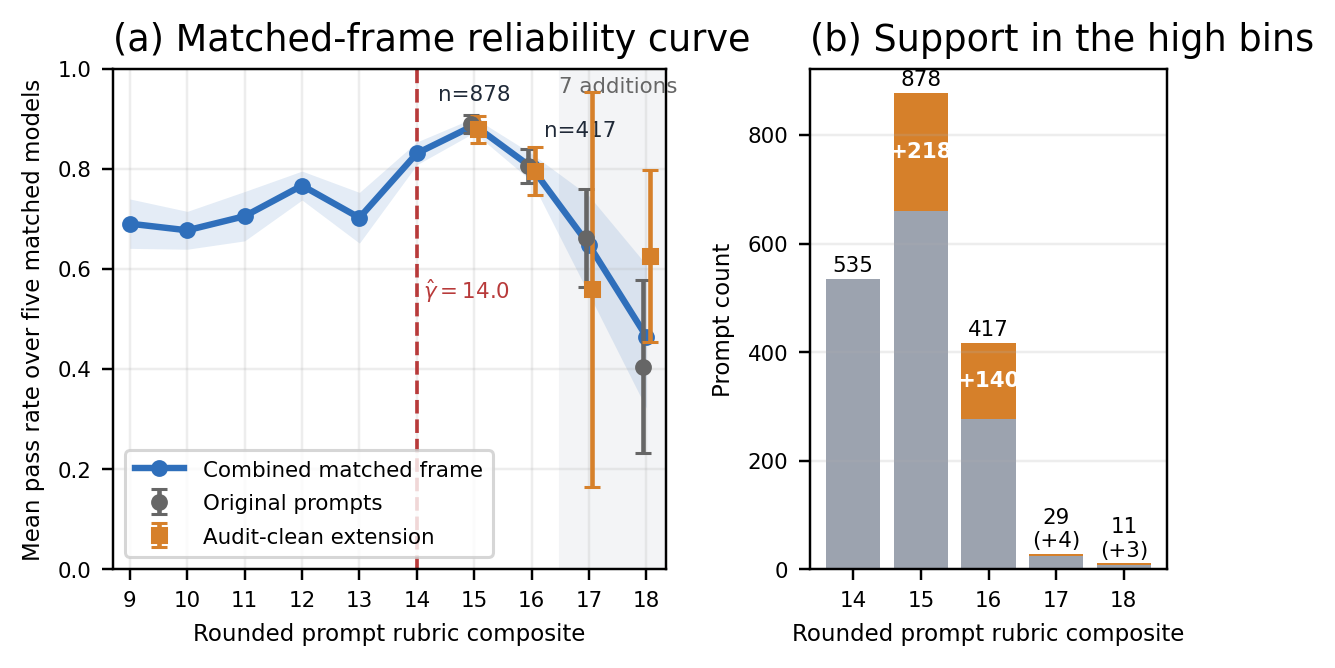
\includegraphics[width=\linewidth]{tail_extension.png}
\caption{Audit-clean extension in a matched five-model frame. (a) Pass rate is first averaged over the five models shared by the original benchmark and extension, then over prompts within display bins, where bin $b$ contains $C_i\in[b-0.5,b+0.5)$. Error bars and the shaded band are prompt-level normal-approximation intervals using $\pm1.96$ standard errors. The dashed line is the same-frame threshold estimated on the unbinned composite. (b) The 365 additions materially raise support at bins 15 and 16. Only 14 additions lie above 16, so bins 17 and 18 remain descriptive.}
\label{fig:tail-extension}
\end{figure}

A separate fixed-version three-model check with Claude Opus 4.6, GPT-5.4, and Gemini 3.1 Pro Preview analyzes the same 150 midrange anchors plus 365 retained tail prompts per model. Their bin-15 pass rates are 0.941, 0.940, and 0.936, and their bin-16 rates are 0.871, 0.850, and 0.845. Only 14 retained tail prompts lie above bin 16, so the extreme-tail shape remains unresolved.

\subsection{Repeated-Sampling Robustness}

On a 359-prompt, four-model subset with five draws per prompt-model cell at temperature 0.8 (7{,}180 scored generations), the mean within-cell standard deviation is 0.064 and the median is zero. The first draw and five-draw mean both select $\hat{\gamma}=14.25$. Their Pearson correlation is 0.960, but this is a part-whole comparison because the first draw contributes to the mean. This local check supports threshold-location stability for the sampled subset; it does not establish universal single-draw reliability.

% =====================================================================
\section{Discussion}
% =====================================================================

\subsection{Interpretation After the IV Diagnostics}

The full six-dimension IV specification does not support causal identification. Its Sargan statistic is $J=411.32$ on five degrees of freedom, and the robust Wooldridge overidentification statistic is 350.59; both reject at machine precision. This is not explained away by sample size. Across 200 random subsamples at each size, mean $J/N$ changes only from 0.102 at $n=250$ to 0.082 at $n=4{,}000$, and 97.5\% of the $n=250$ draws already reject. Under the null, expected $J$ would be about five; the mean at $n=250$ is 25.5.

The dimensions also imply conflicting just-identified coefficients. Data structures is positive ($0.00213$, $p=3.2\times10^{-6}$), while state ($-0.00378$) and composition ($-0.00416$) are strongly negative. Rotating the same space does not repair the disagreement: all overidentified leading-principal-component fits reject, while PC1 alone is just-identified and therefore has no overidentification test. A few post hoc subsets do not reject, such as branching plus edge cases ($p=0.968$, robust first-stage Wald $\chi^2(2)=7{,}570$), but subset search is multiplicity-sensitive and does not validate the original six-dimension IV specification.

What survives is the composite's use as a pre-generation index. Its timing avoids the mechanical failure dependence of generated-output CC, and its association with reference CC, human ratings, paraphrases, and language re-expressions can be evaluated directly. None of those checks turns the index into a causal instrument.

\subsection{What the Breakpoint Means}

The unadjusted mean-pooled breakpoint is a compact description of a nonmonotone curve in a selection-stratified benchmark. It is not a universal difficulty limit. Four results make that boundary especially important. First, task-type controls shrink the gap from 7.6 to 2.1 points and move the estimated location. Second, construction-frame control reverses the selected raw regime gap, and neither frame alone reproduces the pooled increase. Third, median pooling shifts the estimate to 10.75. Fourth, unadjusted model-specific directions differ, and their source sensitivities differ as well. Kimi K2.5 is the clearest downward benchmark-conditioned example; Gemini has a downward but imprecisely localized later-frame change, while Grok-3, GPT-5.4, and Qwen 3.6 Plus reverse direction in the later-frame raw contrast. The leave-one-model-out stability shows that no single model creates the mean-pooled estimate, but it does not remove dependence on the pooling functional or prompt composition. A model-specific $\hat{\gamma}$ therefore estimates a candidate reliability breakpoint for a named model under the constructed frame, index, generation settings, and test protocol. It is not a universal or causal failure threshold.

The 365-prompt extension strengthens the evidence only where it adds support. Bins 15 and 16 closely match the original matched-five-model point estimates, while bins 17 and 18 receive only 11 and three additions. We therefore find similar rates through bin 16 within this frame and leave the extreme tail unresolved.

\subsection{Why a Prompt-Side Index Is Useful}

The central design choice is temporal rather than causal: measure the input before the evaluated system acts. A lexical proxy also has this advantage and may be preferable when transparency or cost dominates. The rubric offers a different tradeoff: six interpretable structural dimensions, ensemble disagreement, and a scale that can be calibrated across raters and prompt variants. The disagreement-enriched two-grader calibration shows that the measurement remains uncertain in this sample and argues for reporting uncertainty rather than treating any single rater as ground truth.

The same pre-generation principle may transfer beyond Python code prompts, but the evidence here is narrow. Java and C++ rescoring preserves the index ordering, while generation and execution remain Python-only. Applications to other textual artifacts would need their own rubric, human calibration, and outcome-specific validation.

\subsection{Implications for Benchmark Design}
Analyses that stratify by generated-output complexity should report how missing and failed outputs enter the metric. A prompt-side score can supplement those plots, provided its sampling frame, rater reliability, and sensitivity to task composition are visible. We recommend reporting the full curve, bin support, alternative pooling choices, and task-type-adjusted results rather than reducing reliability to one average or one cutoff. Such scores are diagnostic summaries, not deployment rules without prospective validation.

% =====================================================================
\section{Limitations}
\label{sec:limitations}
% =====================================================================
% \subsection{Current limitations}

\textbf{Constructed sampling frame.} The benchmark is balanced across bands of a preliminary single-rater score, not the final four-judge index. Its source pool also inherits a 200{,}000-record prefix scan and deliberate high-reference-complexity supplementation. The retained and later-candidate frames differ sharply in score and pass rate, and the source sensitivity shows that their changing mixture explains much of the pooled rebound. The benchmark therefore does not estimate performance under the natural OpenCodeInstruct prompt distribution. Regime means and breakpoint estimates are conditional on the evaluated model or pooling rule, constructed frame, scoring index, generation settings, and unit-test protocol.

\textbf{Scorer dependence and human disagreement.} Systematic LLM-rater bias can propagate into the index. The four-judge ensemble makes disagreement observable but cannot remove common-mode bias. Human-LLM agreement is only moderate on the disagreement-enriched 200-prompt sample and varies substantially by rater.

\textbf{Composition and pooling.} Task-type and construction-frame controls substantially alter the breakpoint, and median pooling also changes its location. The mean-pooled 13.75 estimate should not be read without those sensitivities.

\textbf{Post hoc model exclusion.} AuroraGPT-IT-v4 was removed in a post hoc panel decision without a prespecified eligibility rule and lacks final-frame outputs for 2{,}754 prompts. A like-for-like 22-model sensitivity on the final frame is therefore unavailable.

\textbf{Sparse extreme tail.} The audit-clean extension adds 351 prompts at bins 15 and 16 but only 14 above 16. The endpoint beyond bin 16 remains underpowered.

\textbf{Python execution only.} Java and C++ results test score transfer after re-expression. We did not rerun generation and unit-test execution in those languages.

\textbf{No causal IV claim.} The overidentification restrictions reject even in small subsamples, and candidate instruments imply conflicting coefficients. The 2SLS fits cannot identify a causal effect.

\textbf{Post hoc checks and cross-sectional scope.} The task taxonomy, construction-frame sensitivity, tail extension, human calibration, paraphrase, language, and repeated-sampling checks were added after the initial analysis. They sharpen the evidence but are not preregistered. We also do not track comparable prompts and model families over time.

% =====================================================================
\section{Conclusion}
% =====================================================================

Generated-output cyclomatic complexity is a poor stand-in for prompt structure when failures can produce short or unscorable programs. A prompt-side index avoids that timing problem and supports model-specific reliability-breakpoint estimation in this benchmark. The clearest downward example is Kimi K2.5 near 14.25 after construction-frame control and within the later frame, where raw mean pass is lower above the estimated breakpoint. That estimate remains conditional on the prompt frame, scoring index, generation settings, and test protocol. The mean-pooled result is less stable: task-type controls shrink its gap, construction-frame sensitivity shows that the large rebound is mostly compositional, median pooling moves its location, and model-specific directions differ.

The audit-clean extension closely matches the bin-15 and bin-16 point estimates in a matched five-model frame, while support above bin 16 remains too sparse for a strong claim. Human calibration is moderate, paraphrase and language-transfer checks preserve ordering, and repeated sampling preserves the local threshold estimate. The six candidate instruments fail their joint restrictions, so the contribution is measurement and observational analysis, not causal identification.

For benchmark designers, the practical lesson is modest: supplement output-derived metrics with pre-generation measures, publish the rubric and rater uncertainty, show support counts, and report how task composition and pooling alter the curve.

\vspace{4pt}
\noindent\textbf{Reproducibility.} The anonymous source artifact contains analysis code, locked result summaries, aggregate robustness results, and source tables for the figures. Large prompt and generated-output bundles are retained separately and are not part of the Git snapshot.

% =====================================================================


\begin{thebibliography}{99}

\bibitem{chen2021evaluating}
M.~Chen et al., ``Evaluating Large Language Models Trained on Code,'' \emph{arXiv:2107.03374}, 2021.

\bibitem{austin2021program}
J.~Austin et al., ``Program Synthesis with Large Language Models,'' \emph{arXiv:2108.07732}, 2021.

\bibitem{opencodeinst}
NVIDIA, ``OpenCodeInstruct,'' Hugging Face Datasets, 2025.

\bibitem{wooldridge2010econometric}
J.~M.~Wooldridge, \emph{Econometric Analysis of Cross Section and Panel Data}, 2nd~ed., MIT Press, 2010.

\bibitem{linearmodels}
K.~Sheppard, ``linearmodels: Linear panel, instrumental-variable, asset-pricing, and system-regression models for Python,'' version~7.0, 2025. [Online]. Available: \url{https://bashtage.github.io/linearmodels/}

\bibitem{hansen2000sample}
B.~E.~Hansen, ``Sample Splitting and Threshold Estimation,'' \emph{Econometrica}, vol.~68, no.~3, pp.~575 to 603, 2000.

\bibitem{hansen1982large}
L.~P.~Hansen, ``Large Sample Properties of Generalized Method of Moments Estimators,'' \emph{Econometrica}, vol.~50, no.~4, pp.~1029 to 1054, 1982.

\bibitem{jimenez2023swebench}
C.~E.~Jimenez et al., ``SWE-bench: Can Language Models Resolve Real-World GitHub Issues?'' \emph{arXiv:2310.06770}, 2023.

\bibitem{mccabe1976complexity}
T.~J.~McCabe, ``A Complexity Measure,'' \emph{IEEE Transactions on Software Engineering}, vol.~SE-2, no.~4, pp.~308 to 320, 1976. doi:10.1109/TSE.1976.233837.

\bibitem{lizard}
T.~Yin, ``Lizard: A Simple Code Complexity Analyzer,'' GitHub repository. [Online]. Available: \url{https://github.com/terryyin/lizard}

\bibitem{montgomery2018posttreatment}
J.~M.~Montgomery, B.~Nyhan, and M.~Torres, ``How Conditioning on Posttreatment Variables Can Ruin Your Experiment and What to Do about It,'' \emph{American Journal of Political Science}, vol.~62, no.~3, pp.~760 to 775, 2018. doi:10.1111/ajps.12357.

\bibitem{grafvlachy2024cleaning}
L.~Graf-Vlachy and S.~Wagner, ``Cleaning Up Confounding: Accounting for Endogeneity Using Instrumental Variables and Two-Stage Models,'' \emph{ACM Transactions on Software Engineering and Methodology}, vol.~33, no.~8, article~199, 2024. doi:10.1145/3674730.

\bibitem{siebert2023applications}
J.~Siebert, ``Applications of Statistical Causal Inference in Software Engineering,'' \emph{Information and Software Technology}, vol.~159, article~107198, 2023. doi:10.1016/j.infsof.2023.107198.

\bibitem{liu2023geval}
Y.~Liu et al., ``G-Eval: NLG Evaluation using GPT-4 with Better Human Alignment,'' \emph{arXiv:2303.16634}, 2023.

\bibitem{alpacaeval}
X.~Li et al., ``AlpacaEval: An Automatic Evaluator of Instruction Following Models,'' 2023. [Online]. Available: \url{https://github.com/tatsu-lab/alpaca_eval}

\bibitem{zheng2023judging}
L.~Zheng et al., ``Judging LLM-as-a-Judge with MT-Bench and Chatbot Arena,'' \emph{arXiv:2306.05685}, 2023.

\bibitem{hashimoto2019unifying}
T.~B.~Hashimoto et al., ``Unifying Human and Statistical Evaluation for Natural Language Generation,'' \emph{arXiv:1904.02792}, 2019.

\bibitem{stock2005testing}
J.~H.~Stock and M.~Yogo, ``Testing for Weak Instruments in Linear IV Regression,'' in \emph{Identification and Inference for Econometric Models}, Cambridge Univ.\ Press, 2005, pp.~80 to 108.

\bibitem{bowsher2002reject}
C.~G.~Bowsher, ``On testing overidentifying restrictions in dynamic panel data models,'' \emph{Economics Letters}, vol.~77, no.~2, pp.~211 to 220, 2002.

\end{thebibliography}

\appendix

\section{Additional Econometric Diagnostics}
\label{app:econ-diagnostics}

\subsection{First-stage relevance}

The first-stage regression (\ref{eq:stage1}) on the combined dataset yields a heteroscedasticity-robust Wald statistic of $\chi^2(6)=13{,}611.3$ and a classical joint $F(6,4993)=2{,}265.4$. Partial $R^2$ on generated-output complexity is $0.681$. Per-model robust Wald statistics range from $\chi^2(6)=6{,}053.7$ (GPT-5-mini) to 14{,}693.2 (Mistral Small 2412). The dimensions are strongly relevant to output CC, but relevance does not establish exclusion validity.

\begin{table}[h]
\centering
\caption{First-stage OLS coefficients for candidate rubric dimensions predicting generated-output complexity. Heteroscedasticity-consistent (HC1) standard errors are in parentheses. $N=5{,}000$.}
\label{tab:stage1}
\begin{tabular}{@{}llc@{}}
\toprule
Dimension & $\hat{\pi}$ & SE \\
\midrule
Branching        & $1.090^{***}$  & $(0.238)$ \\
Iteration        & $0.634^{***}$  & $(0.172)$ \\
State            & $2.091^{***}$  & $(0.292)$ \\
Data structures  & $2.851^{***}$  & $(0.138)$ \\
Edge cases       & $6.024^{***}$  & $(0.279)$ \\
Composition      & $-0.766^{**}$  & $(0.291)$ \\
Constant         & $-4.924^{***}$ & $(0.311)$ \\
\midrule
Partial $R^2$                & \multicolumn{2}{c}{0.681} \\
Classical joint $F$          & \multicolumn{2}{c}{2{,}265.4} \\
Robust Wald $\chi^2(6)$      & \multicolumn{2}{c}{13{,}611.3} \\
$N$                          & \multicolumn{2}{c}{5{,}000} \\
\bottomrule
\multicolumn{3}{l}{\footnotesize $^{**}p<0.01$, $^{***}p<0.001$}
\end{tabular}
\end{table}

All six dimensions are individually significant first-stage predictors. \emph{Edge cases} and \emph{data structures} have the largest conditional associations; \emph{composition} is negative after conditioning on the other five dimensions, illustrating substantial shared variance.

\subsection{Overidentification diagnostics}

The Sargan statistic is $411.32$ on $\chi^2(5)$ and the robust Wooldridge statistic is $350.59$; both reject at machine precision. The same pattern appears in every model-specific fit. The restrictions fail well before the full sample size. Table~\ref{tab:overid-subsamples} summarizes 200 random draws at each $n$.

\begin{table}[h]
\centering
\caption{Overidentification under random subsampling. Under the null, $\mathbb{E}[J]\approx5$. Values are means over 200 draws at each subsample size.}
\label{tab:overid-subsamples}
\begin{tabular}{@{}rrrr@{}}
\toprule
$n$ & Mean $J$ & Mean $J/n$ & Share rejecting at 0.05 \\
\midrule
250   & 25.46  & 0.1018 & 0.975 \\
500   & 45.61  & 0.0912 & 1.000 \\
1{,}000 & 86.87  & 0.0869 & 1.000 \\
2{,}000 & 167.48 & 0.0837 & 1.000 \\
3{,}000 & 247.78 & 0.0826 & 1.000 \\
4{,}000 & 329.83 & 0.0825 & 1.000 \\
5{,}000 & 411.32 & 0.0823 & 1.000 \\
\bottomrule
\end{tabular}
\end{table}

The just-identified coefficients disagree in sign: branching $-0.00083$ ($p=0.043$), iteration $-0.00035$ ($p=0.519$), state $-0.00378$ ($p=2.1\times10^{-12}$), data structures $+0.00213$ ($p=3.2\times10^{-6}$), edge cases $-0.00084$ ($p=0.035$), and composition $-0.00416$ ($p<10^{-15}$). The sign disagreement is consistent with the failed joint restrictions.

Principal-component rotation preserves the same disagreement. PC1 explains 78.5\% of the dimension variance and, as the sole instrument in the prompt-level pass-rate-on-mean-output-CC diagnostic, gives $\hat{\beta}=-0.000588$ (SE $=0.000387$, $p=0.129$) with robust first-stage Wald $\chi^2(1)=8{,}489$. Because that fit is just-identified, it has no overidentification test and is a robustness specification rather than a repair. Adding PC2 raises cumulative explained variance to 87.7\% and already rejects ($J=24.44$, $p=7.65\times10^{-7}$); every larger leading-PC specification also rejects, and the full six-PC fit reproduces $J=411.32$ exactly. Under the reported component orientation, PC1 loads broadly across all six dimensions, while PC2 contrasts branching ($+0.54$) and edge cases ($+0.48$) against data structures ($-0.54$) and iteration ($-0.41$).

The post hoc subset search finds five Sargan-nonrejecting specifications: branching plus iteration ($p=0.260$), branching plus edge cases ($p=0.968$), iteration plus edge cases ($p=0.279$), state plus composition ($p=0.282$), and branching plus iteration plus edge cases ($p=0.525$). Their first-stage statistics range from 4{,}652 to 7{,}768. These subsets were selected after examining the same data and are multiplicity-sensitive diagnostics, not validation of the original instrument set.

\subsection{Output-CC regression diagnostics}

\begin{table}[h]
\centering
\caption{Descriptive OLS and candidate-IV 2SLS fits of pass rate on prompt-level mean generated-output CC, averaged over model generations with computable CC. Of 5{,}000 prompts, 4{,}294 have all 21 model values and 706 use fewer. OLS uses HC1 standard errors and 2SLS uses heteroscedasticity-robust standard errors. Because the full instrument set fails overidentification, the 2SLS coefficient is not causal.}
\label{tab:ols-vs-2sls}
\begin{tabular}{@{}lcc@{}}
\toprule
Regressor: generated-output CC & OLS & Candidate-IV 2SLS \\
\midrule
$\hat{\beta}$ & $+0.00087^{**}$ & $-0.00014$ \\
              & $(0.00033)$ & $(0.00038)$ \\
\midrule
Robust first-stage Wald $\chi^2(6)$ & n/a & 13{,}611.3 \\
Partial $R^2$ & n/a & 0.681 \\
$N$ & \multicolumn{2}{c}{5{,}000} \\
\bottomrule
\multicolumn{3}{l}{\footnotesize $^{**}p<0.01$}
\end{tabular}
\end{table}

The direct output-CC slope is small and positive, while the invalid candidate-IV fit is near zero. The failed exclusion restrictions prevent a causal reading of their difference. Separately, a fractional-probit fit of pass rate on the prompt composite gives a marginal effect at the mean of $-0.00193$ (SE $=0.00480$, $p=0.124$); linear OLS on the prompt composite gives $-0.00186$ ($R^2=0.0008$, $p=0.022$). These small global prompt-index slopes are compatible with the visibly nonmonotone conditional curve.

\subsection{Keyword-feature baseline}

Table~\ref{tab:keyword-baseline} compares the keyword-feature baseline and the prompt-side rubric on the main measurement weaknesses. The keyword baseline is an internal lexical proxy computed from prompt text, not a prior published result.

\begin{table}[h]
\centering
\caption{Keyword-feature baseline and prompt-side rubric. Both are measured before generation; the rubric adds explicit dimensions and rater uncertainty, while the lexical proxy is cheaper and deterministic.}
\label{tab:keyword-baseline}
\begin{tabular}{@{}lll@{}}
\toprule
Issue & Keyword baseline & Prompt rubric \\
\midrule
Output-side contamination & Avoided & \textbf{Avoided} \\
Measurement timing        & Before generation & Before generation \\
$\kappa=1$ vs $\kappa=2$  & $\Delta=+0.58$ & $\Delta=+0.61$ \\
Number of features        & 8       & 6 \\
Scoring rule              & Deterministic counts & Four-rater mean \\
Scorer disagreement       & n/a     & observable \\
\bottomrule
\end{tabular}
\end{table}

\section{Per-model Details}
\label{app:per-model}

\begin{figure}[h]
\centering
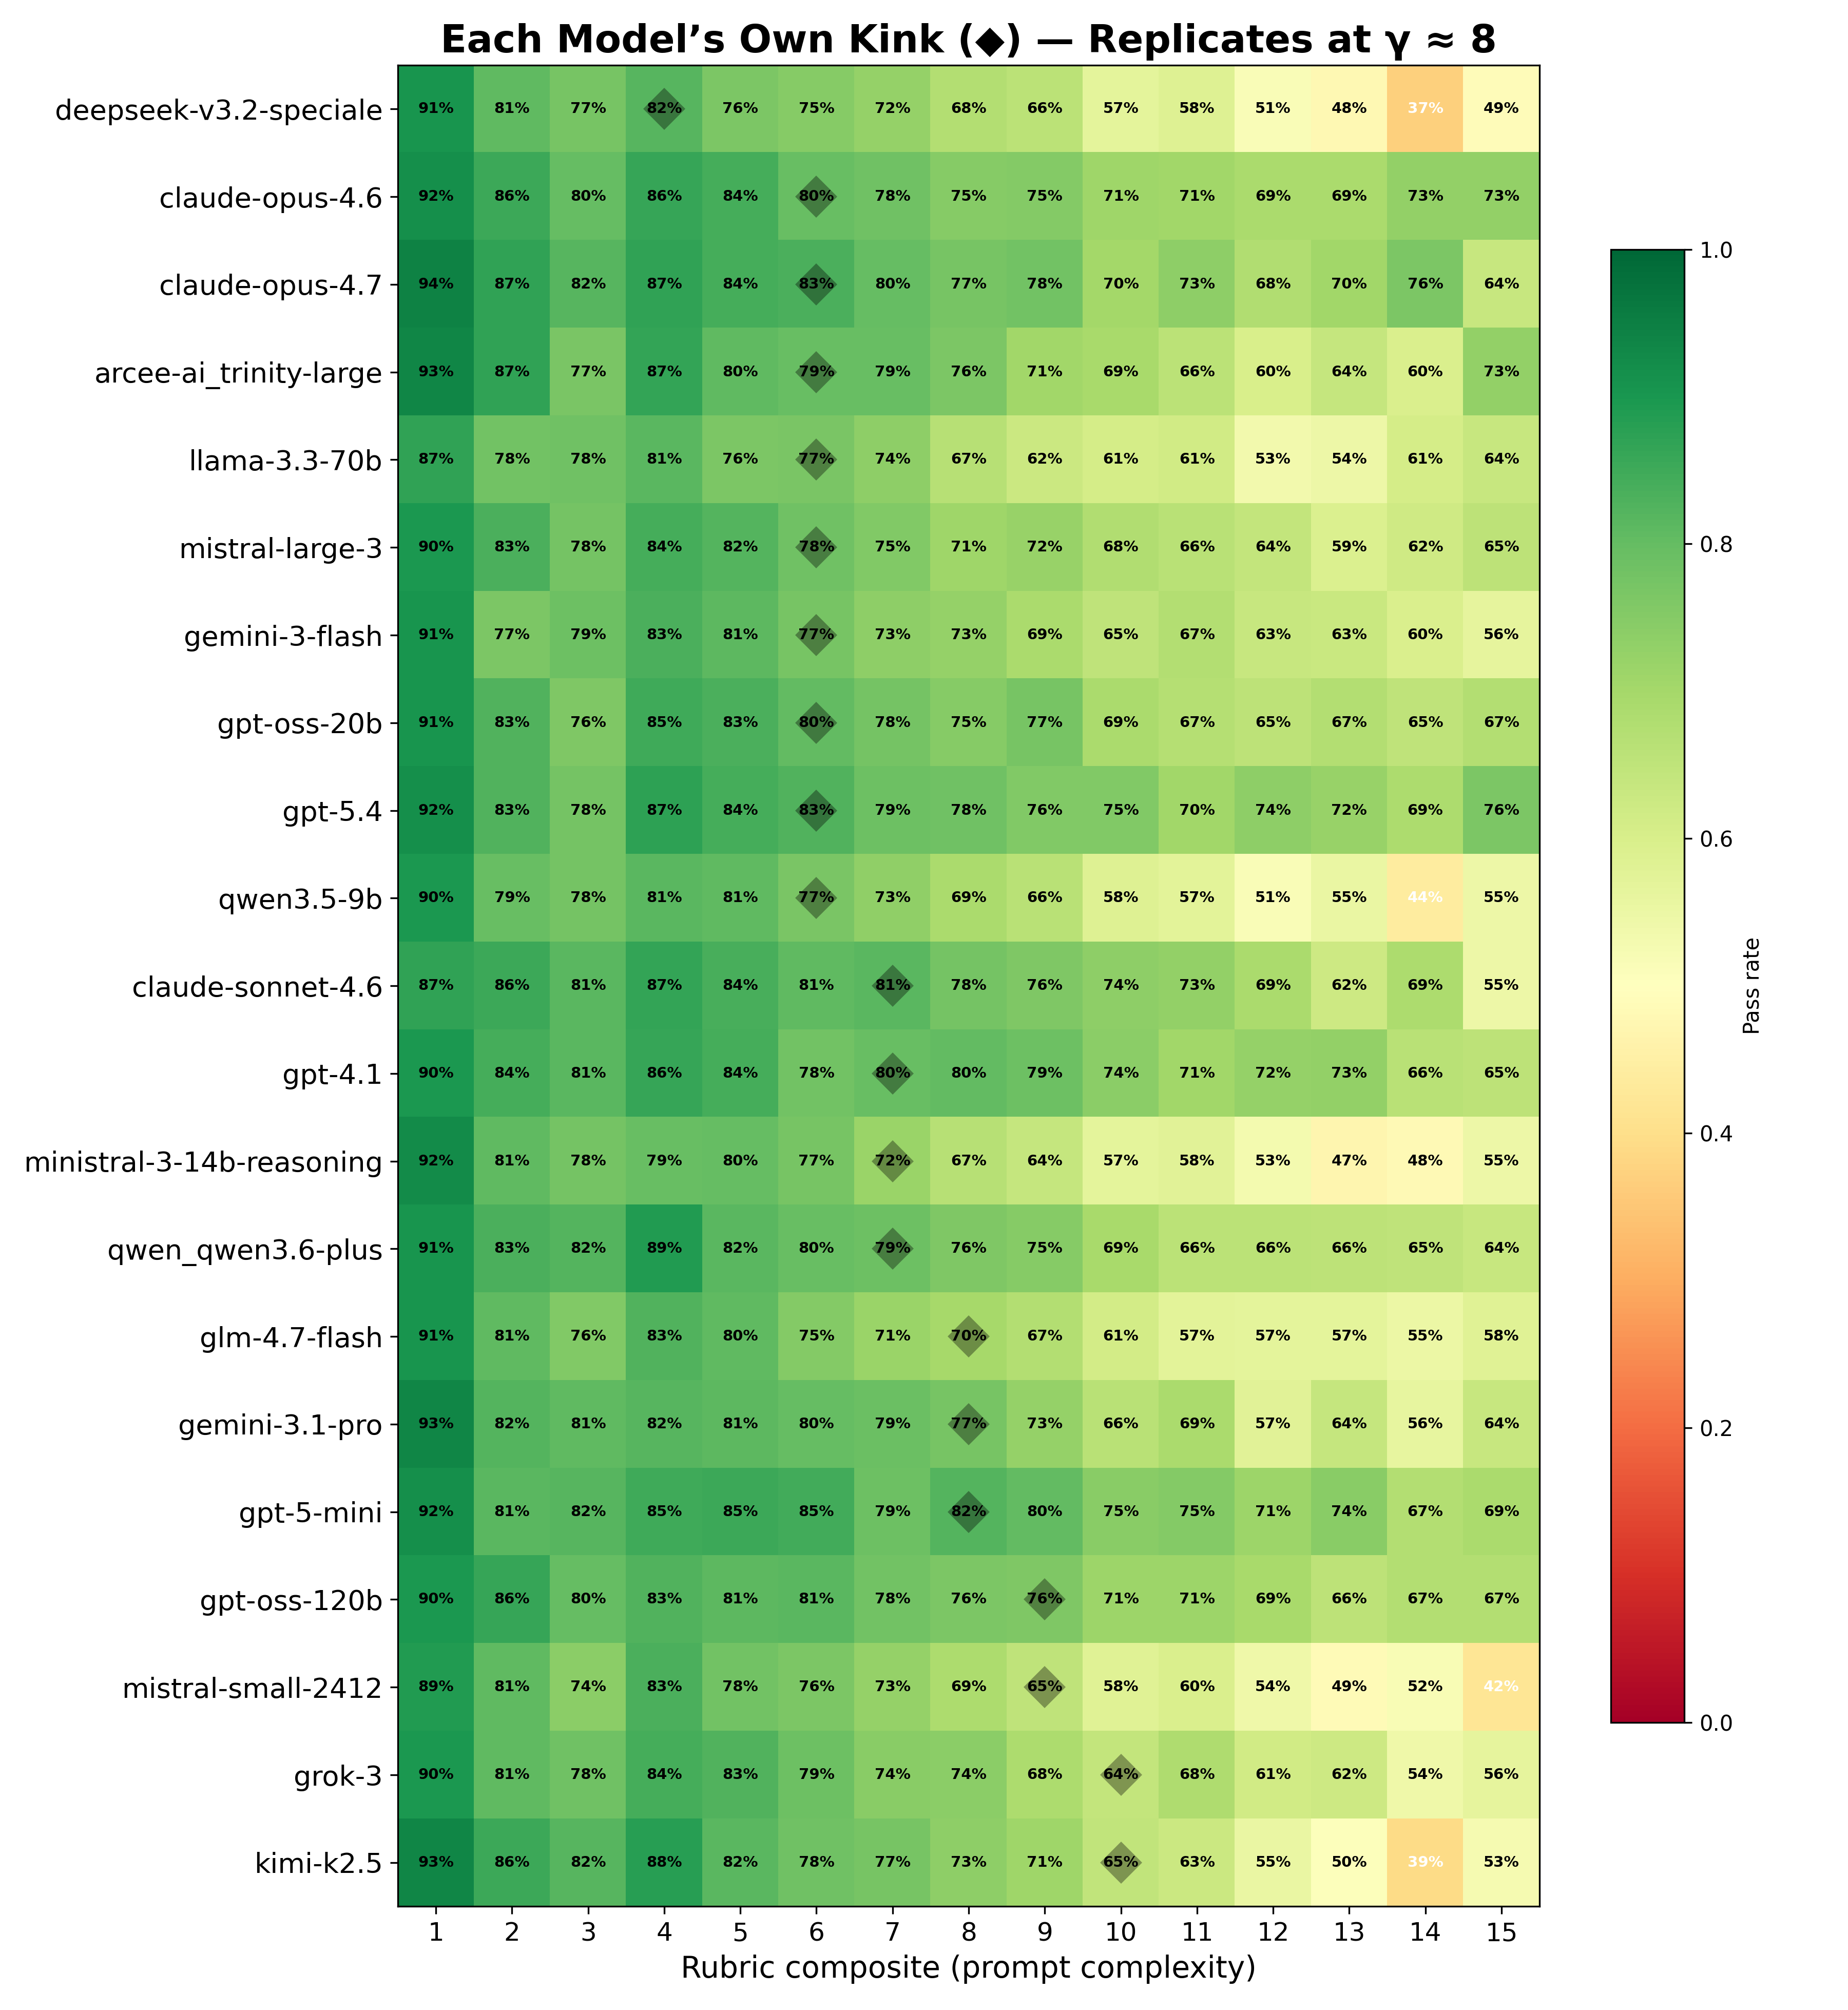
\includegraphics[width=\linewidth]{heatmap_E_per_model_kink.png}
\caption{Model-specific pass rate by prompt-side composite display bin in the original benchmark. Bin $b$ contains $C_i\in[b-0.5,b+0.5)$, so exact half-point boundaries enter the higher bin. Rows are 21 evaluated models and columns are bins 1 to 16. The diamond marks each model's fitted breakpoint in the corresponding display bin. Sparse original bins 0 and 17 to 19 contain 3, 45, 6, and 5 prompts and are omitted.}
\label{fig:heatmap}
\end{figure}

\begin{table}[h]
\centering
\caption{Unadjusted original-benchmark model-specific breakpoint estimates. $\Delta$ is Pass$_{C>\hat{\gamma}}-$Pass$_{C\leq\hat{\gamma}}$ in percentage points. Boot and placebo columns report exceedances out of 500 resamples; zero exceedances imply finite Monte Carlo $p_{\mathrm{MC}}\leq1/501\approx0.002$, not $p=0$. The combined row uses 2{,}000 resamples. These raw regime summaries do not by themselves establish construction-frame-stable failure onsets.}
\label{tab:per-model}
\small
\begin{tabular}{@{}lrrrrrr@{}}
\toprule
Model & $\hat{\gamma}$ & Pass $C\leq\hat{\gamma}$ & Pass $C>\hat{\gamma}$ & $\Delta$ & Boot exc. & Plcb exc. \\
\midrule
Claude Opus 4.6          & 10.50 & 82.7\% & 86.7\% & +3.9 & 0/500 & 0/500 \\
Claude Opus 4.7          & 10.00 & 84.8\% & 86.7\% & +1.9 & 0/500 & 0/500 \\
Claude Sonnet 4.6        & 10.00 & 84.0\% & 85.3\% & +1.3 & 0/500 & 0/500 \\
Trinity-large            & 10.50 & 82.6\% & 85.0\% & +2.4 & 0/500 & 0/500 \\
DeepSeek V3.2            & 10.50 & 78.4\% & 82.3\% & +3.9 & 0/500 & 0/500 \\
GPT-OSS-120B             & 13.75 & 81.4\% & 89.8\% & +8.4 & 0/500 & 0/500 \\
Grok-3                   & 8.25  & 83.6\% & 80.8\% & -2.8 & 0/500 & 0/500 \\
Kimi K2.5                & 14.25 & 77.1\% & 75.3\% & -1.8 & 0/500 & 0/500 \\
Llama 3.3-70B            & 14.00 & 75.2\% & 86.2\% & +11.0 & 0/500 & 0/500 \\
Mistral Large-3          & 13.75 & 80.5\% & 90.4\% & +9.9 & 0/500 & 0/500 \\
GLM 4.7-flash            & 13.75 & 75.7\% & 85.9\% & +10.2 & 0/500 & 0/500 \\
Gemini 3 Flash           & 13.75 & 80.3\% & 89.9\% & +9.6 & 0/500 & 0/500 \\
Gemini 3.1 Pro Preview   & 11.25 & 81.8\% & 74.8\% & -7.0 & 0/500 & 0/500 \\
GPT-4.1                  & 11.25 & 82.8\% & 87.7\% & +4.8 & 0/500 & 0/500 \\
GPT-5-mini               & 10.75 & 85.2\% & 88.4\% & +3.2 & 0/500 & 0/500 \\
GPT-OSS-20B              & 13.75 & 80.4\% & 89.0\% & +8.6 & 0/500 & 0/500 \\
Ministral-3-14B-reasoning & 14.00 & 76.7\% & 84.1\% & +7.4 & 0/500 & 0/500 \\
Mistral Small 2412       & 13.75 & 77.9\% & 86.6\% & +8.6 & 0/500 & 0/500 \\
GPT-5.4                  & 7.75  & 87.4\% & 84.3\% & -3.1 & 0/500 & 0/500 \\
Qwen 3.5-9B              & 14.00 & 75.3\% & 84.5\% & +9.2 & 0/500 & 0/500 \\
Qwen 3.6 Plus            & 7.75  & 85.9\% & 82.1\% & -3.8 & 0/500 & 0/500 \\
\midrule
Combined (21 models)     & 13.75 & 79.9\% & 87.6\% & +7.6 & 0/2{,}000 & 0/2{,}000 \\
\bottomrule
\end{tabular}
\end{table}

\section{Reverse-threshold and Robustness Details}
\label{app:robustness}

\subsection{Reverse-threshold complete cases}

Figure~\ref{fig:sankey} expands the 2-by-2 diagnostic in Figure~\ref{fig:output-cc}. Zero-pass complete cases flow from Lizard complexity on generated code to the prompt composite. Highlighted flows are prompts with composite $>8$ whose failed outputs have CC $\leq10$.

\begin{figure}[h]
\centering
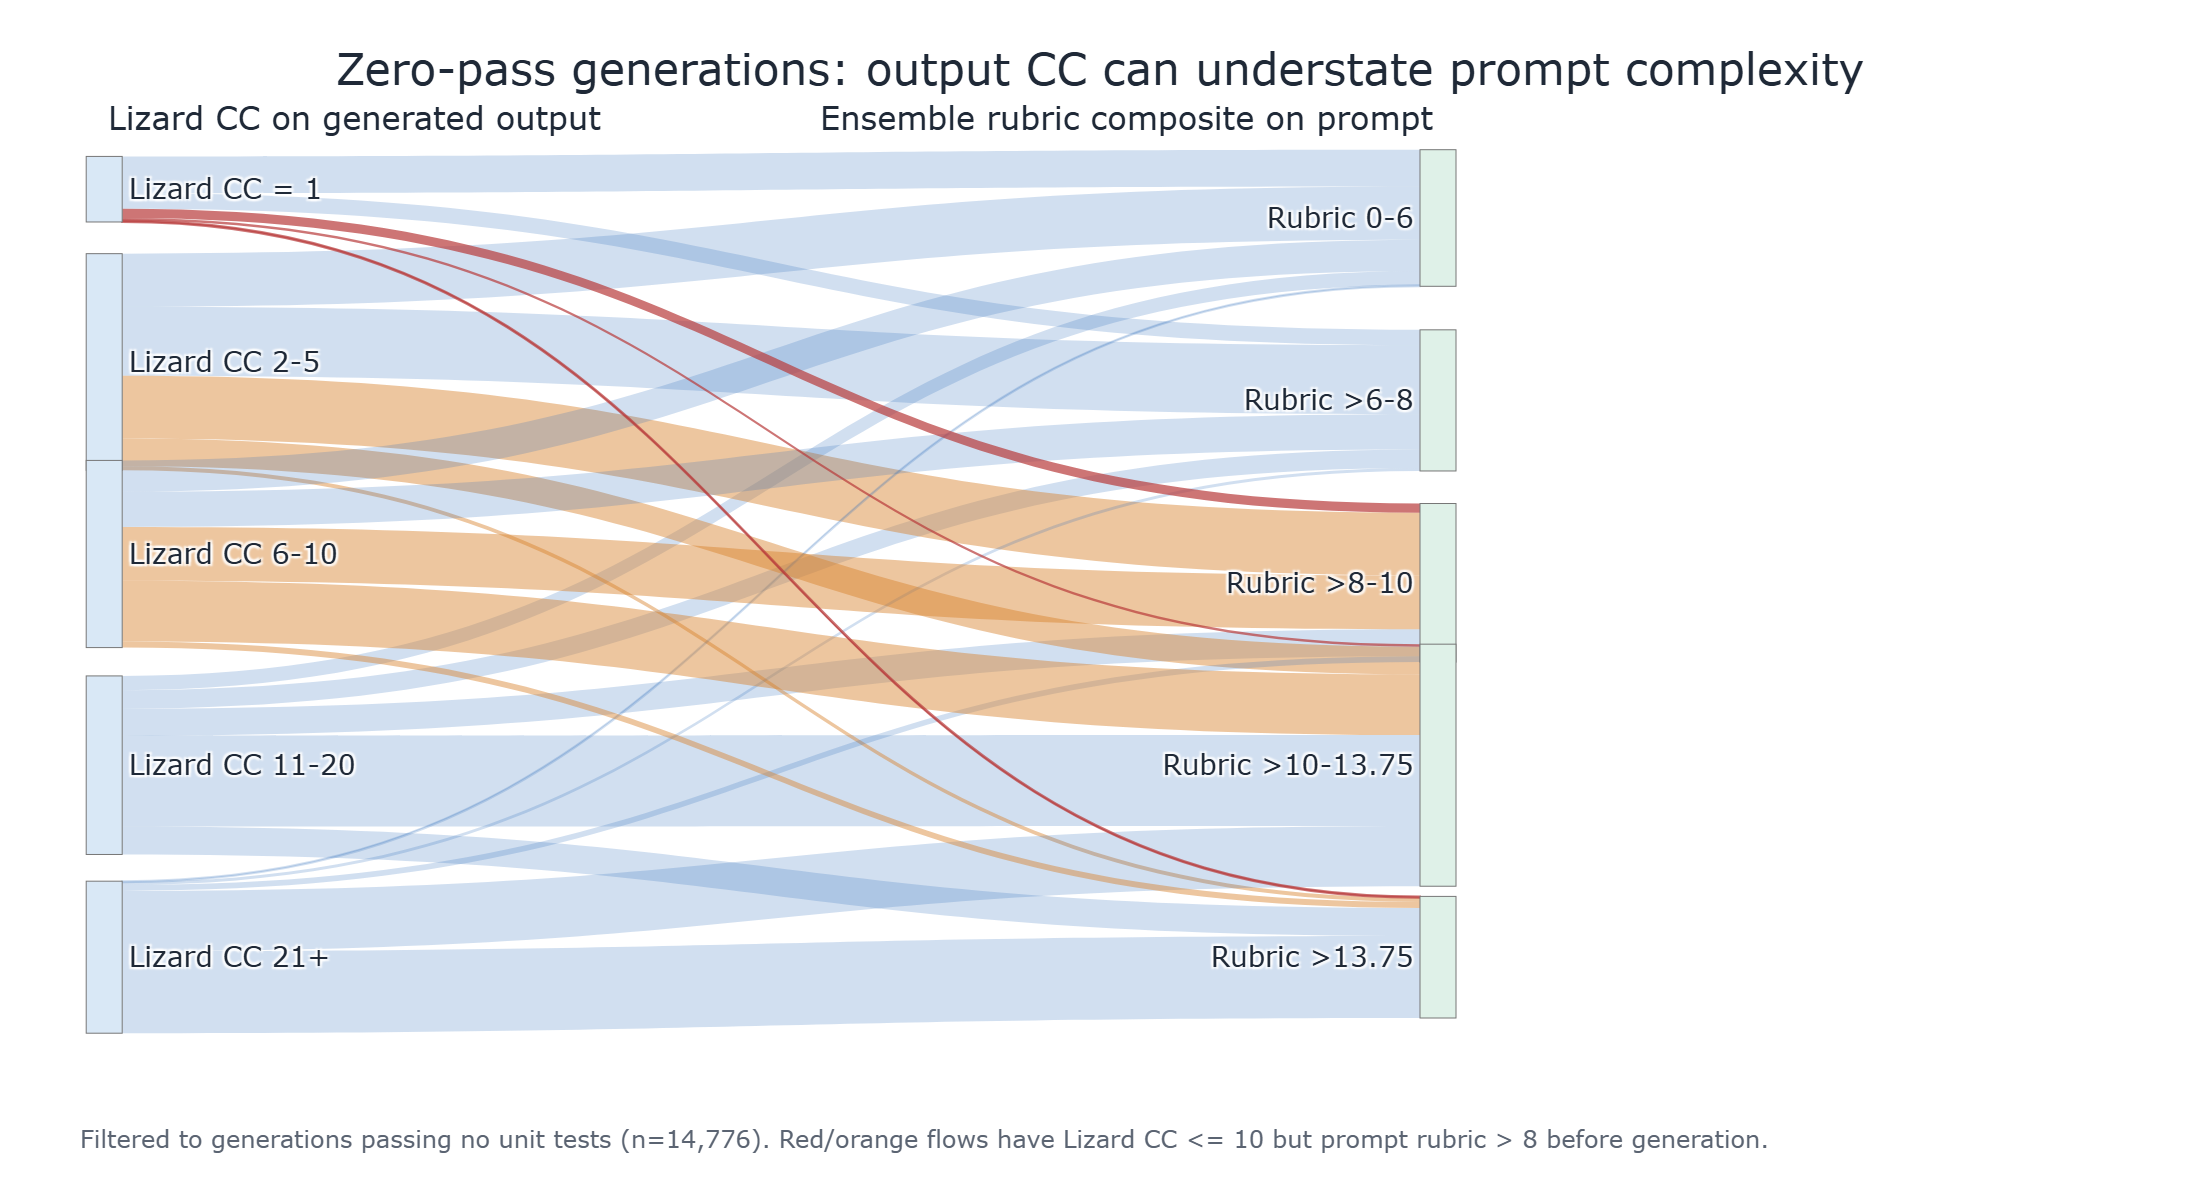
\includegraphics[width=\linewidth]{sankey.png}
\caption{Reverse Threshold Problem among 14{,}776 zero-pass generations with computable Lizard CC. Generated-output complexity is on the left and the pre-generation prompt composite is on the right. Highlighted flows have output CC $\leq10$ and prompt composite $>8$.}
\label{fig:sankey}
\end{figure}

In the revised combined analysis, none of 2{,}000 wild-bootstrap or 2{,}000 shuffled-index placebo statistics reaches the observed $W^*=121.70$. With the standard plus-one correction, each gives $p_{\mathrm{MC}}\leq1/2001<0.001$. For each unadjusted model-specific fit, the observed statistic exceeds all 500 bootstrap and 500 placebo draws, corresponding to $p_{\mathrm{MC}}\leq1/501\approx0.002$.

\subsection{Task-type controls}

The nine fixed categories contain 2{,}005 data-structures/algorithms prompts, 654 array/matrix/grid, 619 numeric/math, 617 string/text, 341 other, 276 stateful simulation, 215 parsing/serialization, 190 logic/validation, and 83 API/library orchestration prompts. On the shared 500-prompt reliability set, pairwise Cohen $\kappa$ ranges from 0.737 to 0.856 and Krippendorff $\alpha=0.787$.

The piecewise composite at 10.75 has $R^2=0.04537$ alone. Task-type fixed effects have $R^2=0.08387$ alone, and their combination has $R^2=0.13640$. Thus the piecewise term adds 0.05253 in-sample predictive $R^2$ beyond the labels. Table~\ref{tab:within-type-j} shows that the IV failure is not localized to one task category.

\begin{table}[h]
\centering
\caption{Full six-dimension Sargan test within task categories having at least 300 prompts.}
\label{tab:within-type-j}
\begin{tabular}{@{}lrrrr@{}}
\toprule
Task category & $n$ & $J$ & $p$ & $J/n$ \\
\midrule
Data structures/algorithms & 2{,}005 & 129.48 & $<10^{-15}$ & 0.0646 \\
Numeric/math               & 619     & 67.52  & $3.4\times10^{-13}$ & 0.1091 \\
Array/matrix/grid          & 654     & 58.90  & $2.1\times10^{-11}$ & 0.0901 \\
String/text                & 617     & 41.59  & $7.1\times10^{-8}$  & 0.0674 \\
Other                      & 341     & 9.58   & 0.088 & 0.0281 \\
\bottomrule
\end{tabular}
\end{table}

\subsection{Construction-frame sensitivity}

All 5{,}000 prompts map to the recorded construction frame. The retained earlier frame contains 2{,}246 prompts and the later candidate frame contains 2{,}754. At the pooled $\hat{\gamma}=13.75$, later candidates account for 39.9\% of the lower regime and 94.7\% of the upper regime. Within the earlier frame, raw pass rate is 0.749 below versus 0.691 above that pooled threshold, with only 73 prompts above. Within the later frame, it is 0.875 versus 0.886. The overlap limitation makes reweighting unstable, so we report the controlled and within-frame fits rather than treating a standardized contrast as definitive.

\begin{table}[h]
\centering
\caption{Unbinned threshold searches within the two construction frames. Regime means are raw summaries at each frame's selected breakpoint.}
\label{tab:source-frame}
\begin{tabular}{@{}lrrrrrr@{}}
\toprule
Frame & $n$ & $\hat{\gamma}$ & sup-Wald & Bootstrap $p$ & Pass low & Pass high \\
\midrule
Retained earlier & 2{,}246 & 7.75 & 3.43 & 0.19 & 0.825 & 0.666 \\
Later candidate & 2{,}754 & 14.25 & 36.71 & $\leq1/301$ & 0.877 & 0.885 \\
\bottomrule
\end{tabular}
\end{table}

For the earlier frame, linear BIC is 1{,}216.0 versus 1{,}224.6 for the piecewise fit. For the later frame, piecewise BIC is $-674.6$ versus $-617.8$ for linear. Across both frames, a model with frame-specific linear slopes has $R^2=0.0991$ and BIC 963.2, compared with $R^2=0.0997$ and BIC 976.9 for the common-frame-effect breakpoint model. Thus nonlinearity remains in the later frame, but the data do not support a common within-frame transition of the pooled magnitude.

\subsection{Pooling and repeated sampling}

Every leave-one-model-out mean-pooled fit selects 13.75. Median pooling selects 10.75, with 0.839 at or below and 0.862 above. Table~\ref{tab:passk} gives the repeated-sampling subset. The subset has 359 prompts, four models, five draws, and 7{,}180 executed generations.

\begin{table}[h]
\centering
\caption{Repeated-sampling threshold check. The first draw is part of the five-draw mean, so $r=0.960$ is a part-whole comparison.}
\label{tab:passk}
\begin{tabular}{@{}lrrrr@{}}
\toprule
Outcome & $\hat{\gamma}$ & sup-Wald & Pass $C\leq\hat{\gamma}$ & Pass $C>\hat{\gamma}$ \\
\midrule
First draw & 14.25 & 10.63 & 0.788 & 0.755 \\
Mean of five draws & 14.25 & 11.42 & 0.785 & 0.750 \\
\bottomrule
\end{tabular}
\end{table}

\subsection{High-complexity extension}

Table~\ref{tab:tail-detail} keeps the original and extension sources separate. Pass rate is first averaged over the five matched models within prompt. The two well-supported comparisons differ by about one percentage point and are not statistically distinguishable. Bins 17 and 18 remain too small for stable comparisons.

\begin{table}[h]
\centering
\caption{Matched-five-model high-bin support and pass rates. Parentheses contain prompt counts.}
\label{tab:tail-detail}
\begin{tabular}{@{}lrrrr@{}}
\toprule
Source & Bin 15 & Bin 16 & Bin 17 & Bin 18 \\
\midrule
Original & 0.894 (850) & 0.808 (257) & 0.718 (45) & 0.450 (6) \\
Audit-clean extension & 0.880 (218) & 0.799 (133) & 0.682 (11) & 0.627 (3) \\
Combined & 0.891 (1{,}068) & 0.805 (390) & 0.711 (56) & 0.509 (9) \\
\midrule
Welch $p$, original vs extension & 0.377 & 0.765 & n/a & n/a \\
\bottomrule
\end{tabular}
\end{table}

The separate fixed-version three-model check analyzes 515 prompts per model: 150 midrange anchors plus 365 audit-clean additions. Claude Opus 4.6, GPT-5.4, and Gemini 3.1 Pro Preview have bin-15 pass rates 0.941, 0.940, and 0.936, and bin-16 rates 0.871, 0.850, and 0.845. The 11 and three prompts in bins 17 and 18 are descriptive only.

\subsection{Human, paraphrase, and language checks}

\begin{table}[h]
\centering
\caption{Prompt-index calibration checks. Human results use a disagreement-enriched stress-test sample. Language results test rescoring after re-expression, not generation or execution.}
\label{tab:measurement-checks}
\begin{tabular}{@{}llrrr@{}}
\toprule
Check & Comparison & $n$ & Pearson $r$ & Additional statistic \\
\midrule
Human, full set & First grader vs ensemble & 200 & 0.408 & ICC$(2,1)=0.395$ \\
Human, overlap & First grader vs ensemble & 50 & 0.613 & mean offset $=-0.69$ \\
Human, overlap & Second grader vs ensemble & 50 & 0.921 & mean offset $=-1.35$ \\
Human, overlap & First vs second grader & 50 & 0.561 & ICC$(2,1)=0.554$ \\
Paraphrase & Original vs plain rewrite & 150 & 0.987 & Spearman $\rho=0.963$ \\
Java & Python vs Java composite & 117 & 0.992 & Java ICC $=0.913$ \\
C++ & Python vs C++ composite & 117 & 0.969 & C++ ICC $=0.882$ \\
\bottomrule
\end{tabular}
\end{table}

The paraphrases have median character length 46.3\% of the originals. Their mean composite shift is $-0.115$ (paired $p=0.031$), with 91.3\% within one point and 99.3\% within two. On the same 117 prompts used for language re-expression, Python inter-judge ICC is 0.912.

\section{Submission artifact and reproducibility details}

For anonymous review, the source artifact includes the six-dimension rubric, model metadata, analysis scripts for the breakpoint, task-control, diagnostic-IV, placebo, and figure pipelines, locked summary outputs, an aggregate robustness summary, and the source CSVs used for the tail-extension and output-CC figures. Large prompt and generated-output bundles are not committed in the Git snapshot, so reproducing model inference and execution requires the separately retained data bundle and provider access.

\textbf{Existing assets and licenses.} The source task pool is OpenCodeInstruct under CC BY 4.0~\cite{opencodeinst}. Generated-output cyclomatic complexity is computed with Lizard 1.21.0 under the MIT License~\cite{lizard}; diagnostic IV estimation uses \texttt{linearmodels} 7.0 under the NCSA License~\cite{linearmodels}. The source repository itself is released under the MIT License.

\textbf{Compute.} The main compute cost is inference: four rubric judges score 5{,}000 prompts each, and 21 evaluated models each generate one answer for every prompt. Open-weight or locally served models are run one model at a time on A100-class GPU workers; serverless/API models are run through provider batch or hosted inference endpoints. Unit-test execution, Lizard scoring, and econometric analysis run on CPU workers. Exact wall times, worker memory, and total compute were not logged consistently across providers, so we do not claim a complete compute accounting.

\textbf{Execution safeguards.} Generated code is executed only inside the benchmark unit-test harness with timeouts and isolated working directories. The source artifact does not release a trained model or a public code-generation service.

\textbf{LLM usage.} LLMs are part of the core methodology as rubric judges and as evaluated code-generation models. LLM-assisted drafting and editing were also used under author supervision; all scientific claims, analysis choices, and final text remain the authors' responsibility.

\newpage
\section*{NeurIPS Paper Checklist}

\begin{enumerate}

\item {\bf Claims}
    \item[] Question: Do the main claims made in the abstract and introduction accurately reflect the paper's contributions and scope?
    \item[] Answer: \answerYes{}
    \item[] Justification: The abstract and Introduction state the central claim: prompt-side complexity measurement prevents output-side failures from being reclassified as easy cases and enables a threshold analysis of code-generation reliability. The stated claims are tied to the 5,000-prompt, 21-model experiment, and the limitations section explicitly bounds generalization.
    \item[] Guidelines:
    \begin{itemize}
        \item The answer NA means that the abstract and introduction do not include the claims made in the paper.
        \item The abstract and/or introduction should clearly state the claims made, including the contributions made in the paper and important assumptions and limitations. A No or NA answer to this question will not be perceived well by the reviewers.
        \item The claims made should match theoretical and experimental results, and reflect how much the results can be expected to generalize to other settings.
        \item It is fine to include aspirational goals as motivation as long as it is clear that these goals are not attained by the paper.
    \end{itemize}

\item {\bf Limitations}
    \item[] Question: Does the paper discuss the limitations of the work performed by the authors?
    \item[] Answer: \answerYes{}
    \item[] Justification: The paper contains a dedicated Limitations section covering scorer dependence, sparse high-complexity support, Python-only scope, the untestability of the exclusion restriction, and pending human calibration.
    \item[] Guidelines:
    \begin{itemize}
        \item The answer NA means that the paper has no limitation while the answer No means that the paper has limitations, but those are not discussed in the paper.
        \item The authors are encouraged to create a separate "Limitations" section in their paper.
        \item The paper should point out any strong assumptions and how robust the results are to violations of these assumptions. The authors should reflect on how these assumptions might be violated in practice and what the implications would be.
        \item The authors should reflect on the scope of the claims made. In general, empirical results often depend on implicit assumptions, which should be articulated.
        \item The authors should reflect on the factors that influence the performance of the approach.
        \item The authors should discuss the computational efficiency of the proposed algorithms and how they scale with dataset size.
    \end{itemize}

\item {\bf Theory assumptions and proofs}
    \item[] Question: For each theoretical result, does the paper provide the full set of assumptions and a complete (and correct) proof?
    \item[] Answer: \answerNA{}
    \item[] Justification: The paper uses standard IV and threshold estimators but does not introduce new theorems or proofs. The identifying assumptions for the empirical IV design are stated in the Background, Methodology, Discussion, and Limitations sections.
    \item[] Guidelines:
    \begin{itemize}
        \item The answer NA means that the paper does not include theoretical results.
        \item All the theorems, formulas, and proofs in the paper should be numbered and cross-referenced.
        \item All assumptions should be clearly stated or referenced in the statement of any theorems.
        \item The proofs can either appear in the main paper or the supplemental material, but if they appear in the supplemental material, the authors are encouraged to provide a short proof sketch to provide intuition.
        \item Inversely, any informal proof provided in the core of the paper should be complemented by formal proofs provided in appendix or supplemental material.
        \item Theorems and Lemmas that the proof relies upon should be properly referenced.
    \end{itemize}

\item {\bf Experimental result reproducibility}
    \item[] Question: Does the paper fully disclose all the information needed to reproduce the main experimental results of the paper to the extent that it affects the main claims and/or conclusions of the paper (regardless of whether the code and data are provided or not)?
    \item[] Answer: \answerYes{}
    \item[] Justification: The Methodology section specifies the prompt source, stratification, scoring rubric, judge ensemble, evaluated panel, unit-test outcome definition, Lizard output-complexity measurement, IV specification, threshold search, and placebo test. The appendix describes the anonymized supplementary artifact containing data, metadata, scores, and scripts needed to reproduce the reported analyses.
    \item[] Guidelines:
    \begin{itemize}
        \item The answer NA means that the paper does not include experiments.
        \item If the paper includes experiments, a No answer to this question will not be perceived well by the reviewers.
        \item If the contribution is a dataset and/or model, the authors should describe the steps taken to make their results reproducible or verifiable.
        \item Depending on the contribution, reproducibility can be supported by code, data, detailed protocols, hyperparameters, random seeds, or sufficient model and system descriptions.
        \item In the case of closed-source models, access to the model may be limited, but there should be some path to reproducing or verifying the results.
    \end{itemize}

\item {\bf Open access to data and code}
    \item[] Question: Does the paper provide open access to the data and code, with sufficient instructions to faithfully reproduce the main experimental results, as described in supplemental material?
    \item[] Answer: \answerYes{}
    \item[] Justification: For double-blind review, an anonymized OpenReview supplementary artifact is provided with prompts, scores, generation metadata, unit-test outcomes, Lizard outputs, analysis scripts, and Croissant metadata. The appendix states that persistent public hosting will be completed for the camera-ready release if accepted.
    \item[] Guidelines:
    \begin{itemize}
        \item The answer NA means that the paper does not include experiments requiring code.
        \item Providing as much information as possible in supplemental material is recommended, but including URLs to data and code is permitted.
        \item While open release is encouraged, authors should also preserve anonymity during double-blind review.
        \item Instructions should contain the environment and commands needed to reproduce the results where applicable.
    \end{itemize}

\item {\bf Experimental setting/details}
    \item[] Question: Does the paper specify all the training and test details (e.g., data splits, hyperparameters, how they were chosen, type of optimizer) necessary to understand the results?
    \item[] Answer: \answerYes{}
    \item[] Justification: The paper does not train a new model, but it specifies the prompt sampling design, judge scoring protocol, model panel, one-generation-per-prompt setting, unit-test execution outcome, Lizard measurement, and econometric estimators. Additional version and execution details are provided in the supplementary artifact described in the appendix.
    \item[] Guidelines:
    \begin{itemize}
        \item The answer NA means that the paper does not include experiments.
        \item The experimental setting should be presented in the core of the paper to a level of detail that is necessary to appreciate the results and make sense of them.
        \item The full details can be provided either with the code, in appendix, or as supplemental material.
    \end{itemize}

\item {\bf Experiment statistical significance}
    \item[] Question: Does the paper report error bars suitably and correctly defined or other appropriate information about the statistical significance of the experiments?
    \item[] Answer: \answerYes{}
    \item[] Justification: The Results section reports robust standard errors, p-values, bootstrap confidence intervals, Hansen sup-Wald tests, placebo tests, and per-model significance checks. Figure captions identify confidence intervals where shown.
    \item[] Guidelines:
    \begin{itemize}
        \item The answer NA means that the paper does not include experiments.
        \item The authors should answer Yes if the results are accompanied by error bars, confidence intervals, or statistical significance tests for the experiments that support the main claims.
        \item The factors of variability that the error bars are capturing should be clearly stated.
        \item The method for calculating error bars should be explained.
    \end{itemize}

\item {\bf Experiments compute resources}
    \item[] Question: For each experiment, does the paper provide sufficient information on the computer resources (type of compute workers, memory, time of execution) needed to reproduce the experiments?
    \item[] Answer: \answerYes{}
    \item[] Justification: The appendix summarizes the compute profile: rubric and panel inference through serverless/API endpoints or one-model-at-a-time A100-class GPU workers, with CPU execution for tests, Lizard scoring, and econometric analysis. The supplementary artifact records model/provider metadata and documents excluded or failed exploratory runs separately from the final panel.
    \item[] Guidelines:
    \begin{itemize}
        \item The answer NA means that the paper does not include experiments.
        \item The paper should indicate the type of compute workers CPU or GPU, internal cluster, or cloud provider, including relevant memory and storage.
        \item The paper should provide the amount of compute required for each of the individual experimental runs as well as estimate the total compute.
        \item The paper should disclose whether the full research project required more compute than the experiments reported in the paper.
    \end{itemize}

\item {\bf Code of ethics}
    \item[] Question: Does the research conducted in the paper conform, in every respect, with the NeurIPS Code of Ethics?
    \item[] Answer: \answerYes{}
    \item[] Justification: The work evaluates code-generation reliability using programming prompts and generated code, and does not collect personal data, deploy a model, or target protected populations. The paper discusses limitations, reproducibility, artifact access, and responsible release considerations.
    \item[] Guidelines:
    \begin{itemize}
        \item The answer NA means that the authors have not reviewed the NeurIPS Code of Ethics.
        \item If the authors answer No, they should explain the special circumstances that require a deviation from the Code of Ethics.
        \item The authors should make sure to preserve anonymity where applicable.
    \end{itemize}

\item {\bf Broader impacts}
    \item[] Question: Does the paper discuss both potential positive societal impacts and negative societal impacts of the work performed?
    \item[] Answer: \answerYes{}
    \item[] Justification: The Introduction, Discussion, Limitations, and Conclusion discuss positive uses for model selection, benchmark design, and deployment guardrails, as well as risks from overgeneralization, scorer bias, and false confidence in complex code-generation settings.
    \item[] Guidelines:
    \begin{itemize}
        \item The answer NA means that there is no societal impact of the work performed.
        \item If the authors answer NA or No, they should explain why their work has no societal impact or why the impact discussion is not applicable.
        \item If there are negative societal impacts, the authors should discuss possible mitigation strategies.
    \end{itemize}

\item {\bf Safeguards}
    \item[] Question: Does the paper describe safeguards that have been put in place for responsible release of data or models that have a high risk for misuse?
    \item[] Answer: \answerNA{}
    \item[] Justification: The paper does not release a trained model or public code-generation service. The appendix nevertheless states execution safeguards for generated code: unit-test harness isolation, timeouts, and release of benchmark artifacts rather than an interactive model.
    \item[] Guidelines:
    \begin{itemize}
        \item The answer NA means that the paper poses no such risks.
        \item Released models that have a high risk for misuse should describe usage guidelines, restrictions, or safety filters.
        \item Datasets scraped from the Internet could pose safety risks; authors should describe how they avoided releasing unsafe content.
        \item We recognize that providing effective safeguards is challenging, but authors are encouraged to make a best faith effort.
    \end{itemize}

\item {\bf Licenses for existing assets}
    \item[] Question: Are the creators or original owners of assets (e.g., code, data, models), used in the paper, properly credited and are the license and terms of use explicitly mentioned and properly respected?
    \item[] Answer: \answerYes{}
    \item[] Justification: The paper cites OpenCodeInstruct, Lizard, linearmodels, and the evaluated model families where used. The appendix states that the supplementary artifact records dependency versions and license information and separates existing assets from derived benchmark outputs.
    \item[] Guidelines:
    \begin{itemize}
        \item The answer NA means that the paper does not use existing assets.
        \item The authors should cite the original paper that produced the code package or dataset.
        \item The authors should state which version of the asset is used and, if possible, include a URL.
        \item The name of the license should be included for each asset.
        \item For existing datasets that are re-packaged, both the original license and the license of the derived asset should be provided.
    \end{itemize}

\item {\bf New assets}
    \item[] Question: Are new assets introduced in the paper well documented and is the documentation provided alongside the assets?
    \item[] Answer: \answerYes{}
    \item[] Justification: The new assets are the locked benchmark subset metadata, rubric scores, model generation metadata, unit-test outcomes, Lizard measurements, and analysis scripts. The appendix states that these are documented in the anonymized supplementary artifact with Croissant metadata, and that persistent public hosting will accompany the camera-ready release if accepted.
    \item[] Guidelines:
    \begin{itemize}
        \item The answer NA means that the paper does not release new assets.
        \item Researchers should communicate the details of the dataset/code/model as part of their submissions via structured templates.
        \item The paper should discuss whether and how consent was obtained from people whose asset is used.
        \item At submission time, remember to anonymize your assets if applicable.
    \end{itemize}

\item {\bf Crowdsourcing and research with human subjects}
    \item[] Question: For crowdsourcing experiments and research with human subjects, does the paper include the full text of instructions given to participants and screenshots, if applicable, as well as details about compensation (if any)?
    \item[] Answer: \answerNA{}
    \item[] Justification: The paper does not involve crowdsourcing or human-subject data collection. The scoring judges are LLM systems, and informal manuscript feedback is not a human-subject experiment.
    \item[] Guidelines:
    \begin{itemize}
        \item The answer NA means that the paper does not involve crowdsourcing nor research with human subjects.
        \item Including this information in the supplemental material is fine, but if the main contribution involves human subjects, then as much detail as possible should be included in the main paper.
        \item According to the NeurIPS Code of Ethics, workers involved in data collection, curation, or other labor should be paid at least the minimum wage in the country of the data collector.
    \end{itemize}

\item {\bf Institutional review board (IRB) approvals or equivalent for research with human subjects}
    \item[] Question: Does the paper describe potential risks incurred by study participants, whether such risks were disclosed to the subjects, and whether Institutional Review Board (IRB) approvals (or an equivalent approval/review based on the requirements of your country or institution) were obtained?
    \item[] Answer: \answerNA{}
    \item[] Justification: No human-subject research or crowdsourcing experiment is conducted, so IRB or equivalent review is not applicable.
    \item[] Guidelines:
    \begin{itemize}
        \item The answer NA means that the paper does not involve crowdsourcing nor research with human subjects.
        \item Depending on the country in which research is conducted, IRB approval or equivalent may be required for any human subjects research.
        \item We recognize that the procedures for this may vary significantly between institutions and locations, and we expect authors to adhere to the NeurIPS Code of Ethics and the guidelines for their institution.
        \item For initial submissions, do not include any information that would break anonymity, such as the institution conducting the review.
    \end{itemize}

\item {\bf Declaration of LLM usage}
    \item[] Question: Does the paper describe the usage of LLMs if it is an important, original, or non-standard component of the core methods in this research? Note that if the LLM is used only for writing, editing, or formatting purposes and does not impact the core methodology, scientific rigor, or originality of the research, declaration is not required.
    \item[] Answer: \answerYes{}
    \item[] Justification: LLM usage is central to the paper: out-of-panel LLMs score prompts with the rubric, and a 21-model LLM panel is evaluated for code-generation reliability. The appendix also declares LLM-assisted drafting and editing under author supervision.
    \item[] Guidelines:
    \begin{itemize}
        \item The answer NA means that the core method development in this research does not involve LLMs as any important, original, or non-standard components.
        \item Please refer to the NeurIPS LLM policy in the handbook for what should or should not be described.
    \end{itemize}

\end{enumerate}


\end{document}
